\chapter{A Grand Apparatus}\label{ch:lhc_cms}
\begin{aquote}{Fran\c{c}ois Englert, CMS: The Art of Science, 2016}
    A glance at the ATLAS and CMS detectors at CERN reveals their beauty...
    These detectors are the modern cathedrals of the rational world created by scientists, experimentalists, and theoreticians. 
\end{aquote}

\section{The Large Hadron Collider}
The Large Hadron Collider (LHC) is the largest particle accelerator ever built. 
Its most striking feature is a 27 km ring buried 100 m beneath the Franco-Swiss border (Fig.~\ref{fig:lhc_depth}) in which two beams of protons (or heavy ions like lead), after going through several smaller stages (Fig.~\ref{fig:cern_complex}), are accelerated to 99.9999991\% of the speed of light in opposite directions. 
The beams are steered by thousands of magnets, including 1232 superconducting dipole magnets (Fig.~\ref{fig:lhc_dipole}), placed along the circumference of the ring. 
At various points, the proton beams are directed towards each other, allowing the protons to collide. 
These collision points are surrounded by enormous, multi-layered particle detectors which record snapshots of the collisions. 

\begin{figure}[htb]
    \centering
    \subfloat{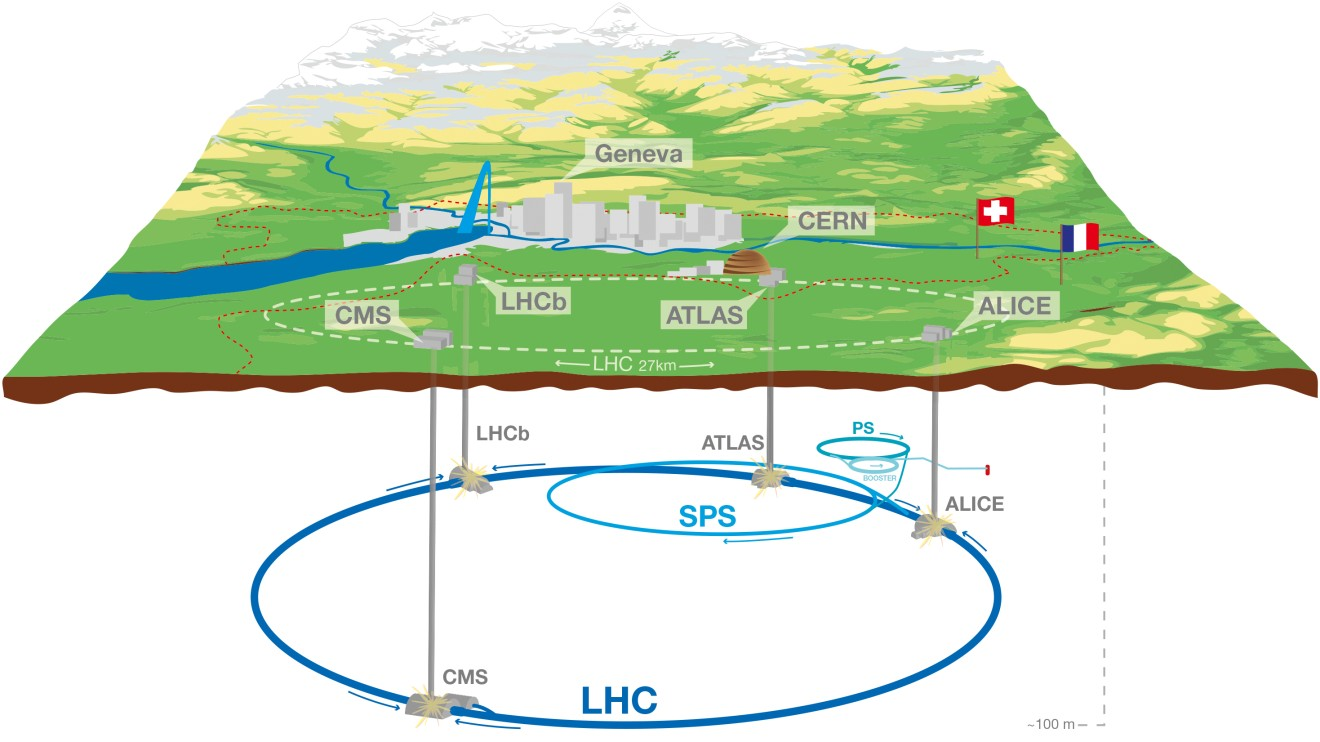
\includegraphics[width=0.45\textwidth,valign=c]{fig/lhc/lhc_depth.jpg}}\quad
    \subfloat{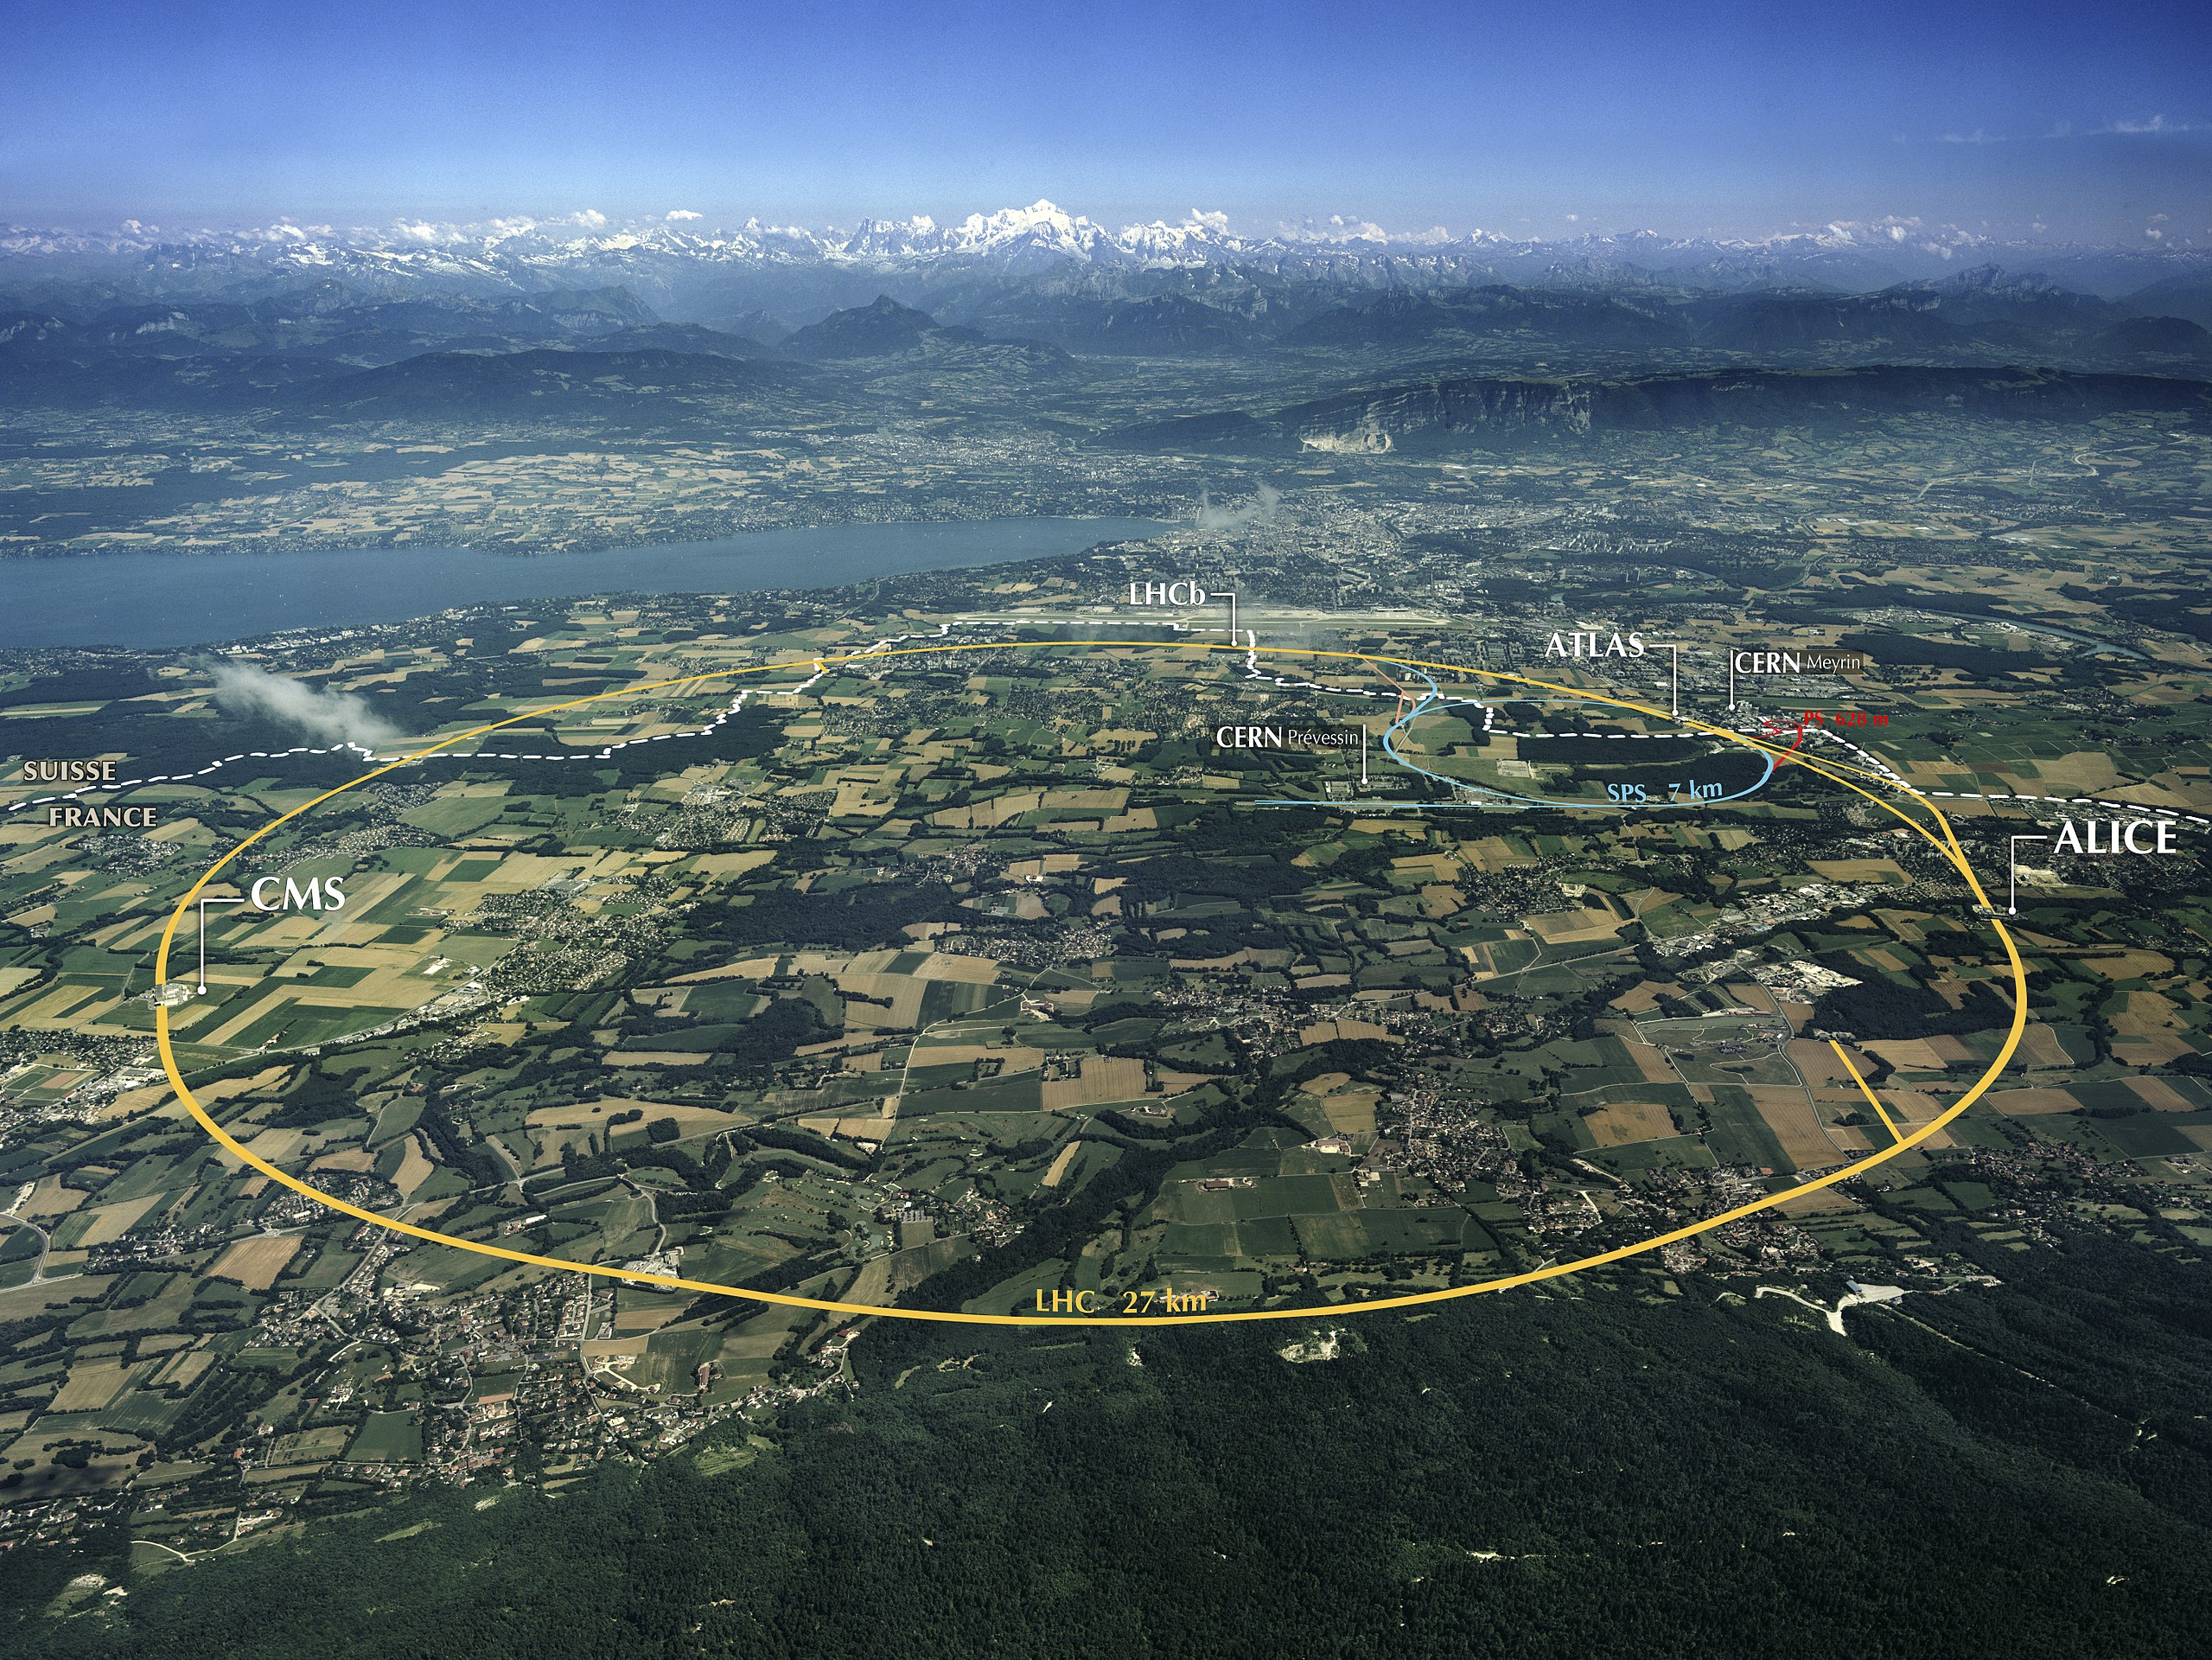
\includegraphics[width=0.45\textwidth,valign=c]{fig/lhc/cern_aerial_view.jpg}}
    \caption[A diagram illustrating the depth of the LHC beneath the surface, from Ref.~\cite{Servicegraphique:1708849}, and an aerial photograph of the entire CERN complex, from Ref.~\cite{Maximilien:1295244}.]{
        A diagram illustrating the depth of the LHC beneath the surface (left), from Ref.~\cite{Servicegraphique:1708849}, and an aerial photograph of the entire CERN complex (right), from Ref.~\cite{Maximilien:1295244}. 
        The SPS and LHC tunnels illustrated in both figures. 
    }
    \label{fig:lhc_depth}
\end{figure}

\begin{figure}[!htb]
    \centering
    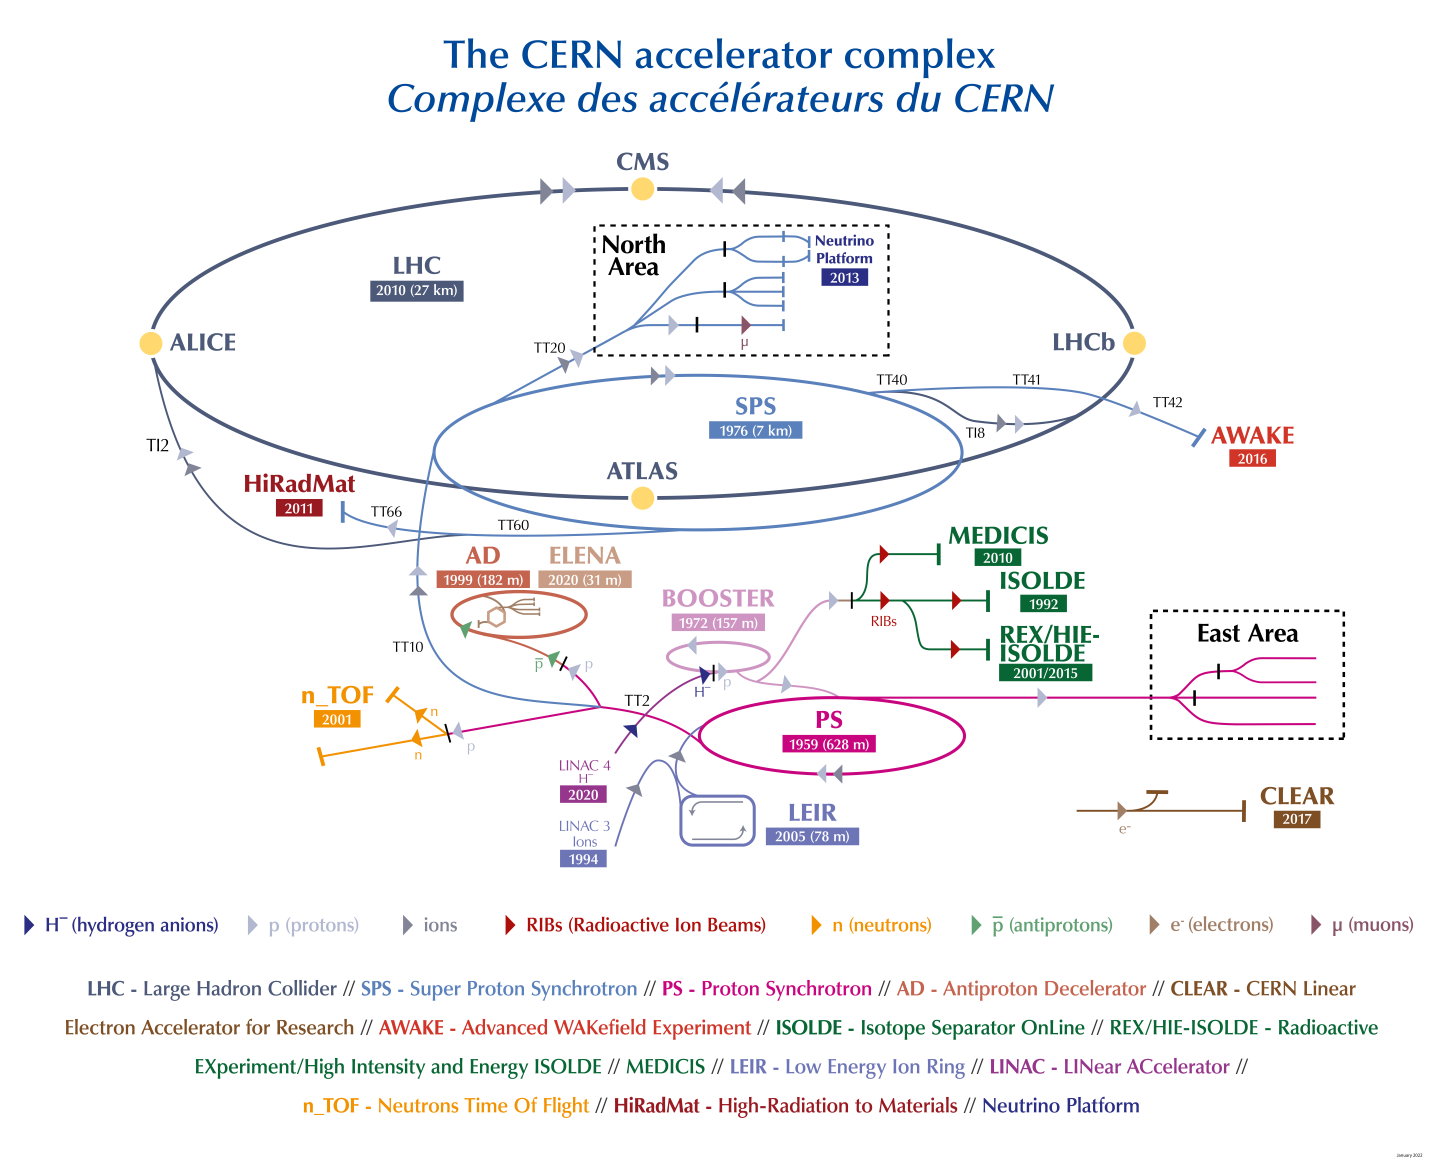
\includegraphics[width=0.95\textwidth]{fig/lhc/lhc_complex.png}
    \caption[The CERN complex illustrated in detail, from Ref.~\cite{Lopienska:2800984}]{
        The CERN complex illustrated in detail, from Ref.~\cite{Lopienska:2800984}. 
        The different stages of particle acceleration can be seen in detail, described here for protons. 
        First, negative hydrogen ions (H$^-$) generated by LINAC 4 are fed into BOOSTER, which strips the electrons from the H$^-$ ions, leaving only the protons, and accelerates them to 2\GeV. 
        Next, the Proton Synchrotron (PS) accelerates the protons to 26\GeV. 
        The PS feeds into the Super Proton Synchrotron (SPS) which further accelerates them to to 450\GeV. 
        Finally, the protons are fed into the LHC, which accelerates them to a final energy of 7\TeV. 
    }
    \label{fig:cern_complex}
\end{figure}

\begin{figure}[htb]
    \centering
    \subfloat{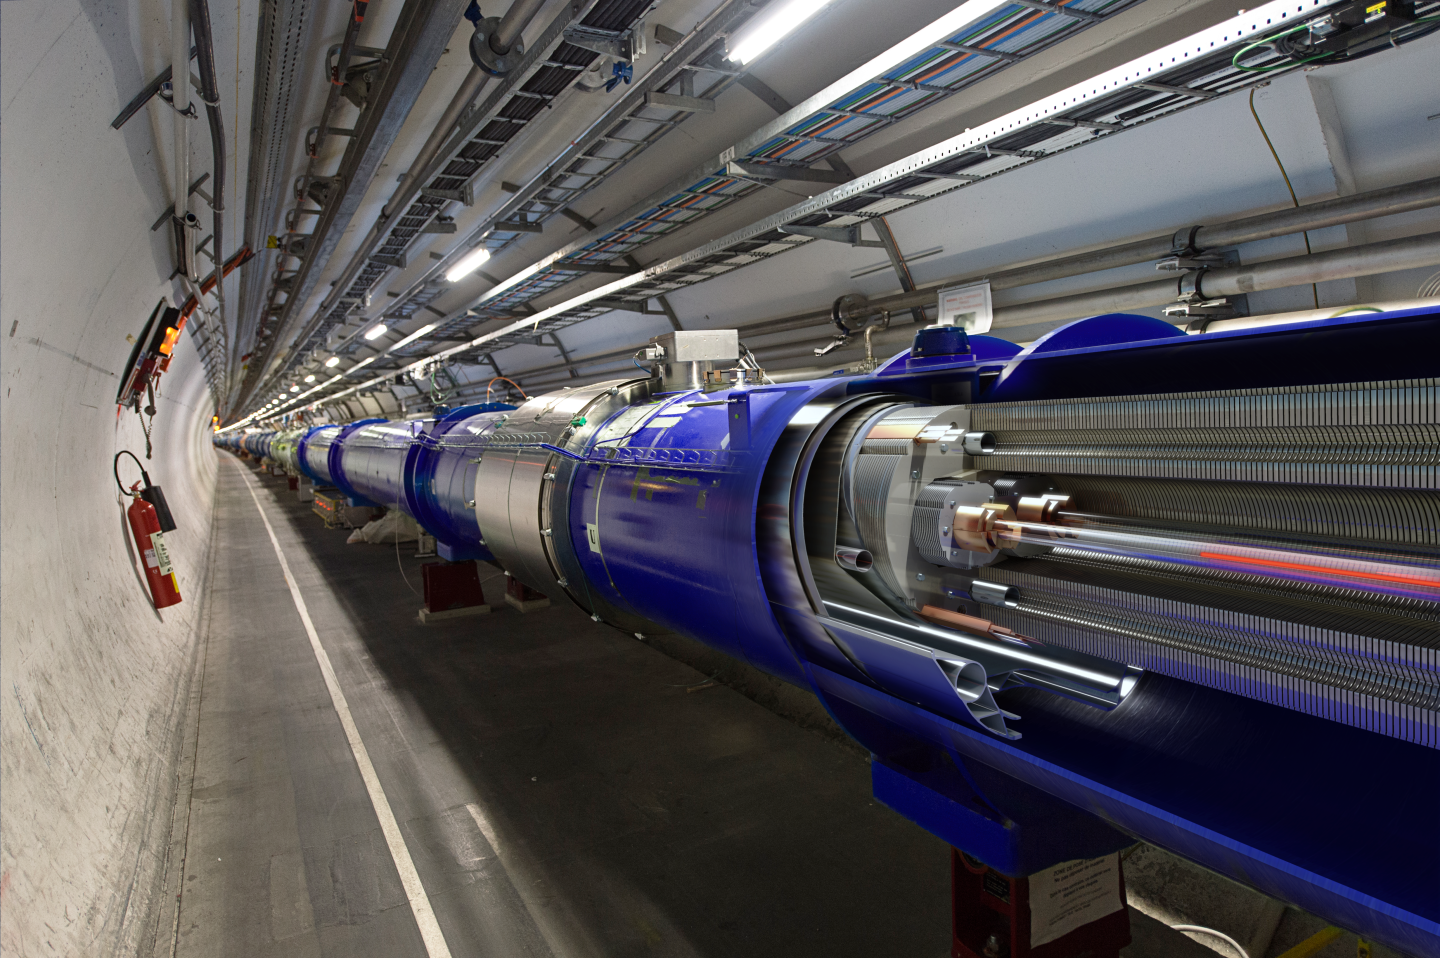
\includegraphics[width=0.475\textwidth,valign=c]{fig/lhc/dipole_cutaway.png}}\quad
    \subfloat{\includegraphics[width=0.425\textwidth,valign=c]{fig/lhc/dipole_jguiang.png}}
    \caption[A cutaway diagram illustrating the internals of a dipole magnet inside the LHC tunnel, from Ref.~\cite{Dominguez:1741036}, and a photograph of a decommissioned dipole magnet with a physicist for scale]{
        A cutaway diagram illustrating the internals of a dipole magnet inside the LHC tunnel (left), from Ref.~\cite{Dominguez:1741036}, and a photograph of a decommissioned dipole magnet with a physicist for scale (right).
    }
    \label{fig:lhc_dipole}
\end{figure}

The protons are accelerated in bunches, composed of approximately 115 billion protons each, so when the bunches are brought together (called a ``bunch crossing''), over 200 billion protons are brought very close together.
However, only a small portion of them actually collide. 
During ``Run 2'' of the LHC from 2016 to 2018, for instance, there were 30 proton-proton (pp) collisions per bunch crossing on average (e.g. Fig.~\ref{fig:normal_pu}), typically with only one interesting collision (the ``primary vertex'') amongst them. 
A collision is deemed interesting if it initiates a process that a physicist at the LHC wants to study (e.g. Fig.~\ref{fig:vbswh_feynman}), or if it looks like such a process, at least---the uninteresting collisions are called ``pileup.'' 
To increase our odds of producing something truly interesting, the bunch crossings are spaced close together, with only 25 nanoseconds of separation. 
To put this into context, the speed of light is roughly 1 ft/ns, so the next bunch crossing will occur before the light from a screen on one side of the CMS control room can reach the eyes of someone standing on the other side (approximately 39 feet~\cite{CMSP5Layout}).

\subsection{Collision energy}
The collision energy, often written as $\sqrt{s}$, is measured in electronvolts (eV), the standard unit of energy in particle physics---at LHC scales, teraelectronvolts (\TeVns), or trillions of eV, are the relevant units. 
In Run I of the LHC (2009--2013) the collision energy was ramped up to a maximum of 8\TeV, much lower than what the LHC was designed for. % TODO: citation needed
This was done out of an abundance of caution due to the fact that the LHC exploded when it was first turned on in 2008. % TODO: citation needed
Then, in Run II (2016--2018), the collision energy was increased to 13\TeV. 
Over the course of Run III, the collision energy will be ramped up to 14\TeV, where it will be held for the remainder of the LHC's lifetime. 
At 7\TeV per proton beam, each bunch has roughly 7 times the kinetic energy of a flying mosquito with a mass ten trillion times smaller. 

\subsection{Luminosity}
The luminosity (\Lumi) is a measure of an accelerator's ability to initiate the desired particle interactions~\cite{Herr:941318}. 
It is thus measured in the inverse units of a cross-section, namely cm$^{-2}$ or inverse barns (b$^{-1}$)---or, at LHC scales, inverse femptobarns (\fbinv).
At the LHC, \Lumi is a measure of the ability to initiate pp collisions. 
Immediately, it is clear that \Lumi should be some function of time: the longer we let the beams collide, the more pp collisions produced. 
This is called the \textit{instantaneous} luminosity, or how many interactions are initiated at any one time. 
We can also consider the \textit{integrated} luminosity, or the total number of interactions initiated over some period of time---as the name suggests, this is simply an integral of the instantaneous luminosity. 
Put simply, the integrated luminosity represents the rate at which interactions occur at the LHC, while the integrated luminosity is a compact shorthand for how many interactions occurred at the LHC during some period of data-taking. 
For example, with the LHC operating at an instantaneous luminosity of $\Lumi = 1\times10^{34}$ cm$^{-2}$s$^{-1}$, given the pp inelastic scattering cross-section at 13\TeV ($\sigma = 71.3$ millibarns~\cite{CMS-PAS-FSQ-15-005}), we can expect $\Lumi\times\sigma = 713$ million pp collisions per second, or 11.24 quadrillion pp collisions over 6 months. 
Importantly, a more specific cross-section $\sigma$---the cross-section for a Higgs boson to be produced in a pp collision, for instance---can be used. 

Based on intuition, we can guess that the luminosity must be a function of the number of protons in a bunch, the bunch spacing, and the exact dynamics of the bunch crossing. 
Indeed, at the LHC, we define the instantaneous luminosity as follows:
\begin{equation}
    \Lumi = \gamma\frac{n_\mathrm{b}N^2f_\text{rev}}{4\pi\beta^{*}\epsilon_\mathrm{n}}R
\end{equation}
where $n_\mathrm{b}$ is the number of bunches per beam, $N$ is the number of protons per bunch, and $f_\text{rev}$ is the frequency at which bunches revolve around the LHC ring, while $\gamma$ comes from special relativity and $\beta^{*}$, $R$, and $\epsilon_\mathrm{n}$ represent physical properties of the proton beams~\cite{Aberle:2749422}. 
Therefore, in order to modify the rate at which interactions may occur, we have several parameters that we can tune.

\section{The Compact Muon Solenoid}\label{sec:cms}
The Compact Muon Solenoid (CMS) Experiment is one of two general purpose LHC experiments, the other being the ATLAS\footnotemark{} Experiment, among the four major experiments supported by the LHC~\cite{LHCWeb}, where the other two are more specialized: ALICE, for studying heavy ion collisions, and LHCb, for studying b quarks. 
\footnotetext{Whereas ATLAS is, putting it politely, a rather creative acronym: ``A Toroidal LHC ApparatuS.''}
Compared to ATLAS, which stands at a mighty $46\times25\times25$ meters in dimension, CMS is ``compact'' at a stout $21\times15\times15$ m, with a dedicated muon system and one of the world's largest solenoids~\cite{ATLASWeb, CMSWeb}. 
See Fig.~\ref{fig:cms_labeled} for its exact specifications, and Figures~\ref{fig:cms_pics} and \ref{fig:cms_jguiang} for some beauty shots. 

\begin{figure}[htb]
    \centering
    \includegraphics[width=0.9\textwidth]{fig/cms/cms_labeled.jpg}
    \caption{
        A detailed cutaway diagram of CMS, from Ref.~\cite{Sakuma:2665537}, with each subdetector labeled with its name and some of its characteristics. 
    }
    \label{fig:cms_labeled}
\end{figure}

\begin{figure}[htb]
    \centering
    \subfloat{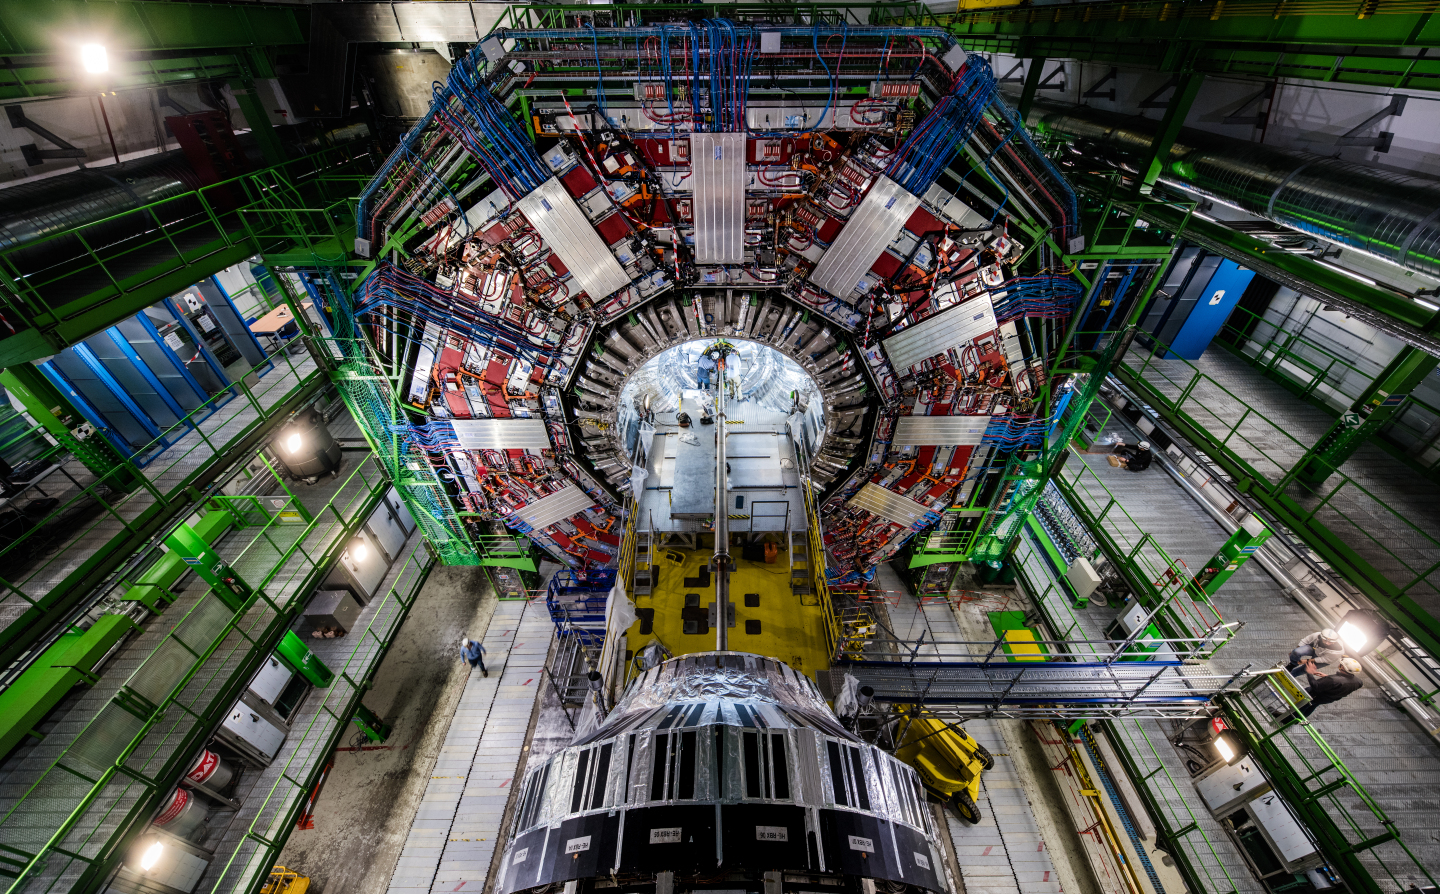
\includegraphics[width=0.465\textwidth]{fig/cms/cms_picture1.jpg}}\quad
    \subfloat{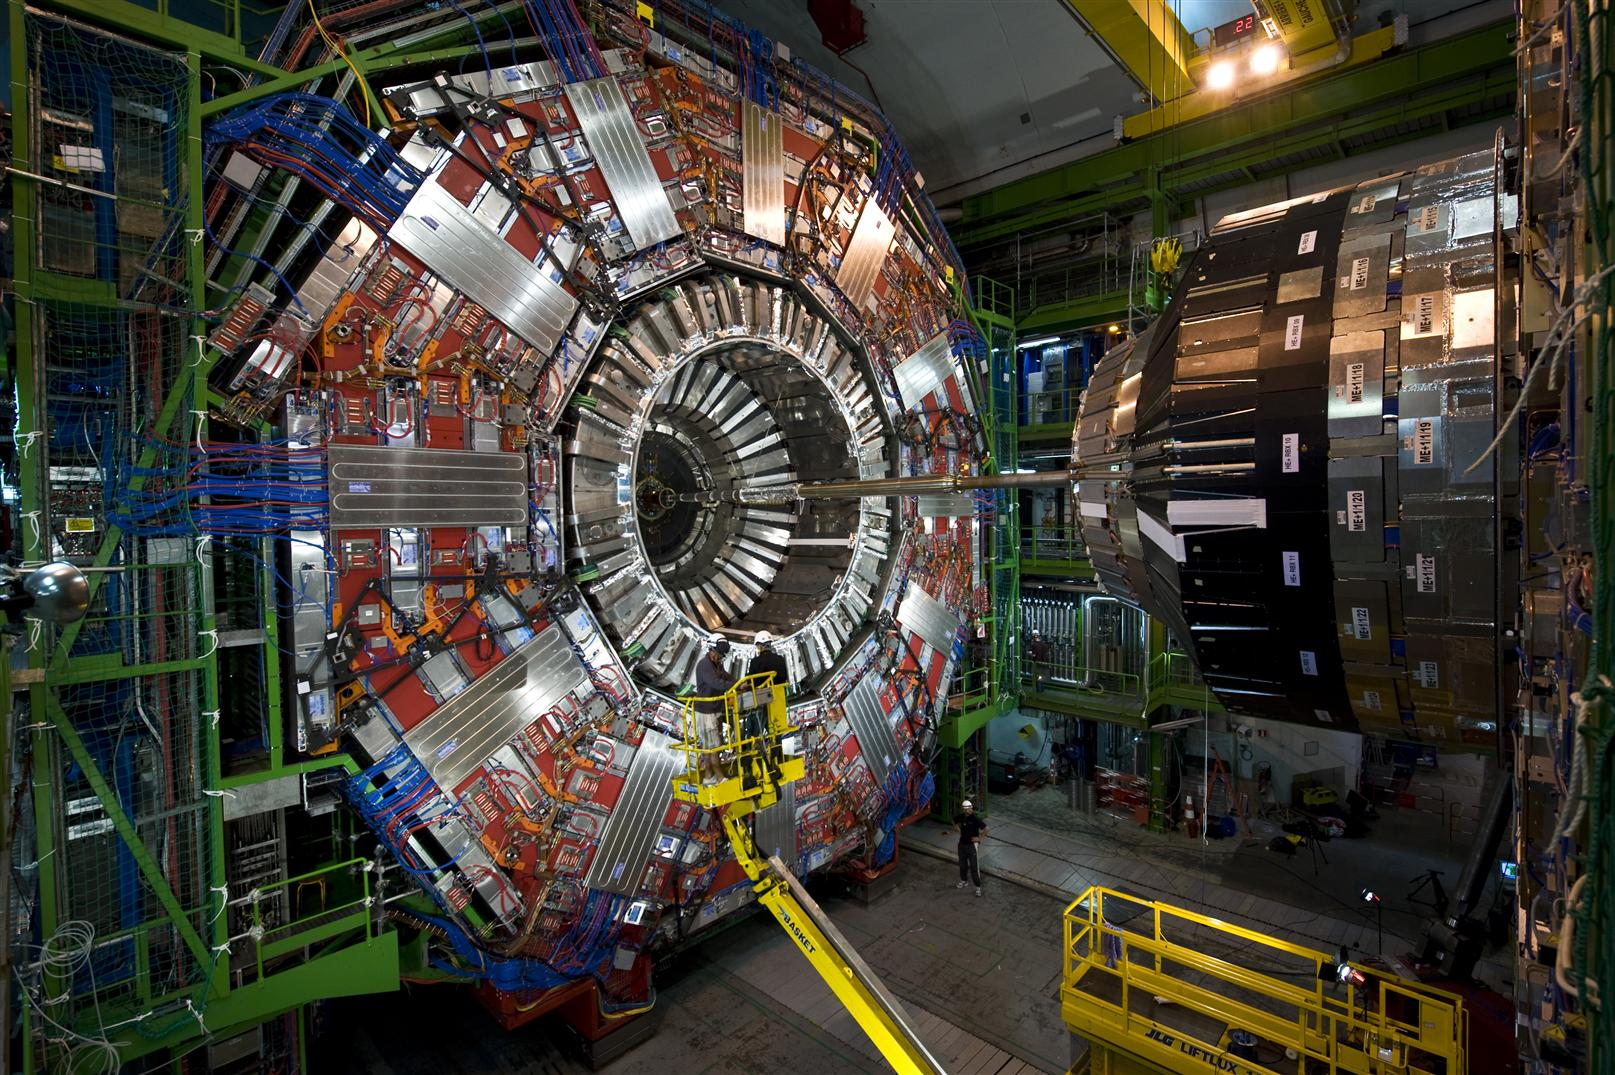
\includegraphics[width=0.435\textwidth]{fig/cms/cms_picture2.jpg}}
    \caption[CMS with one of the endcaps separated from the main body of the experiment, pictured from the top and side]{
        CMS in all of its glory, with one of the endcaps separated from the main body of the experiment, pictured from the top (left), from Ref.~\cite{Brice:2254952}, and side (right), from Ref.~\cite{Maximilien:1133594}. 
    }
    \label{fig:cms_pics}
\end{figure}

\begin{figure}[htb]
    \centering
    \subfloat{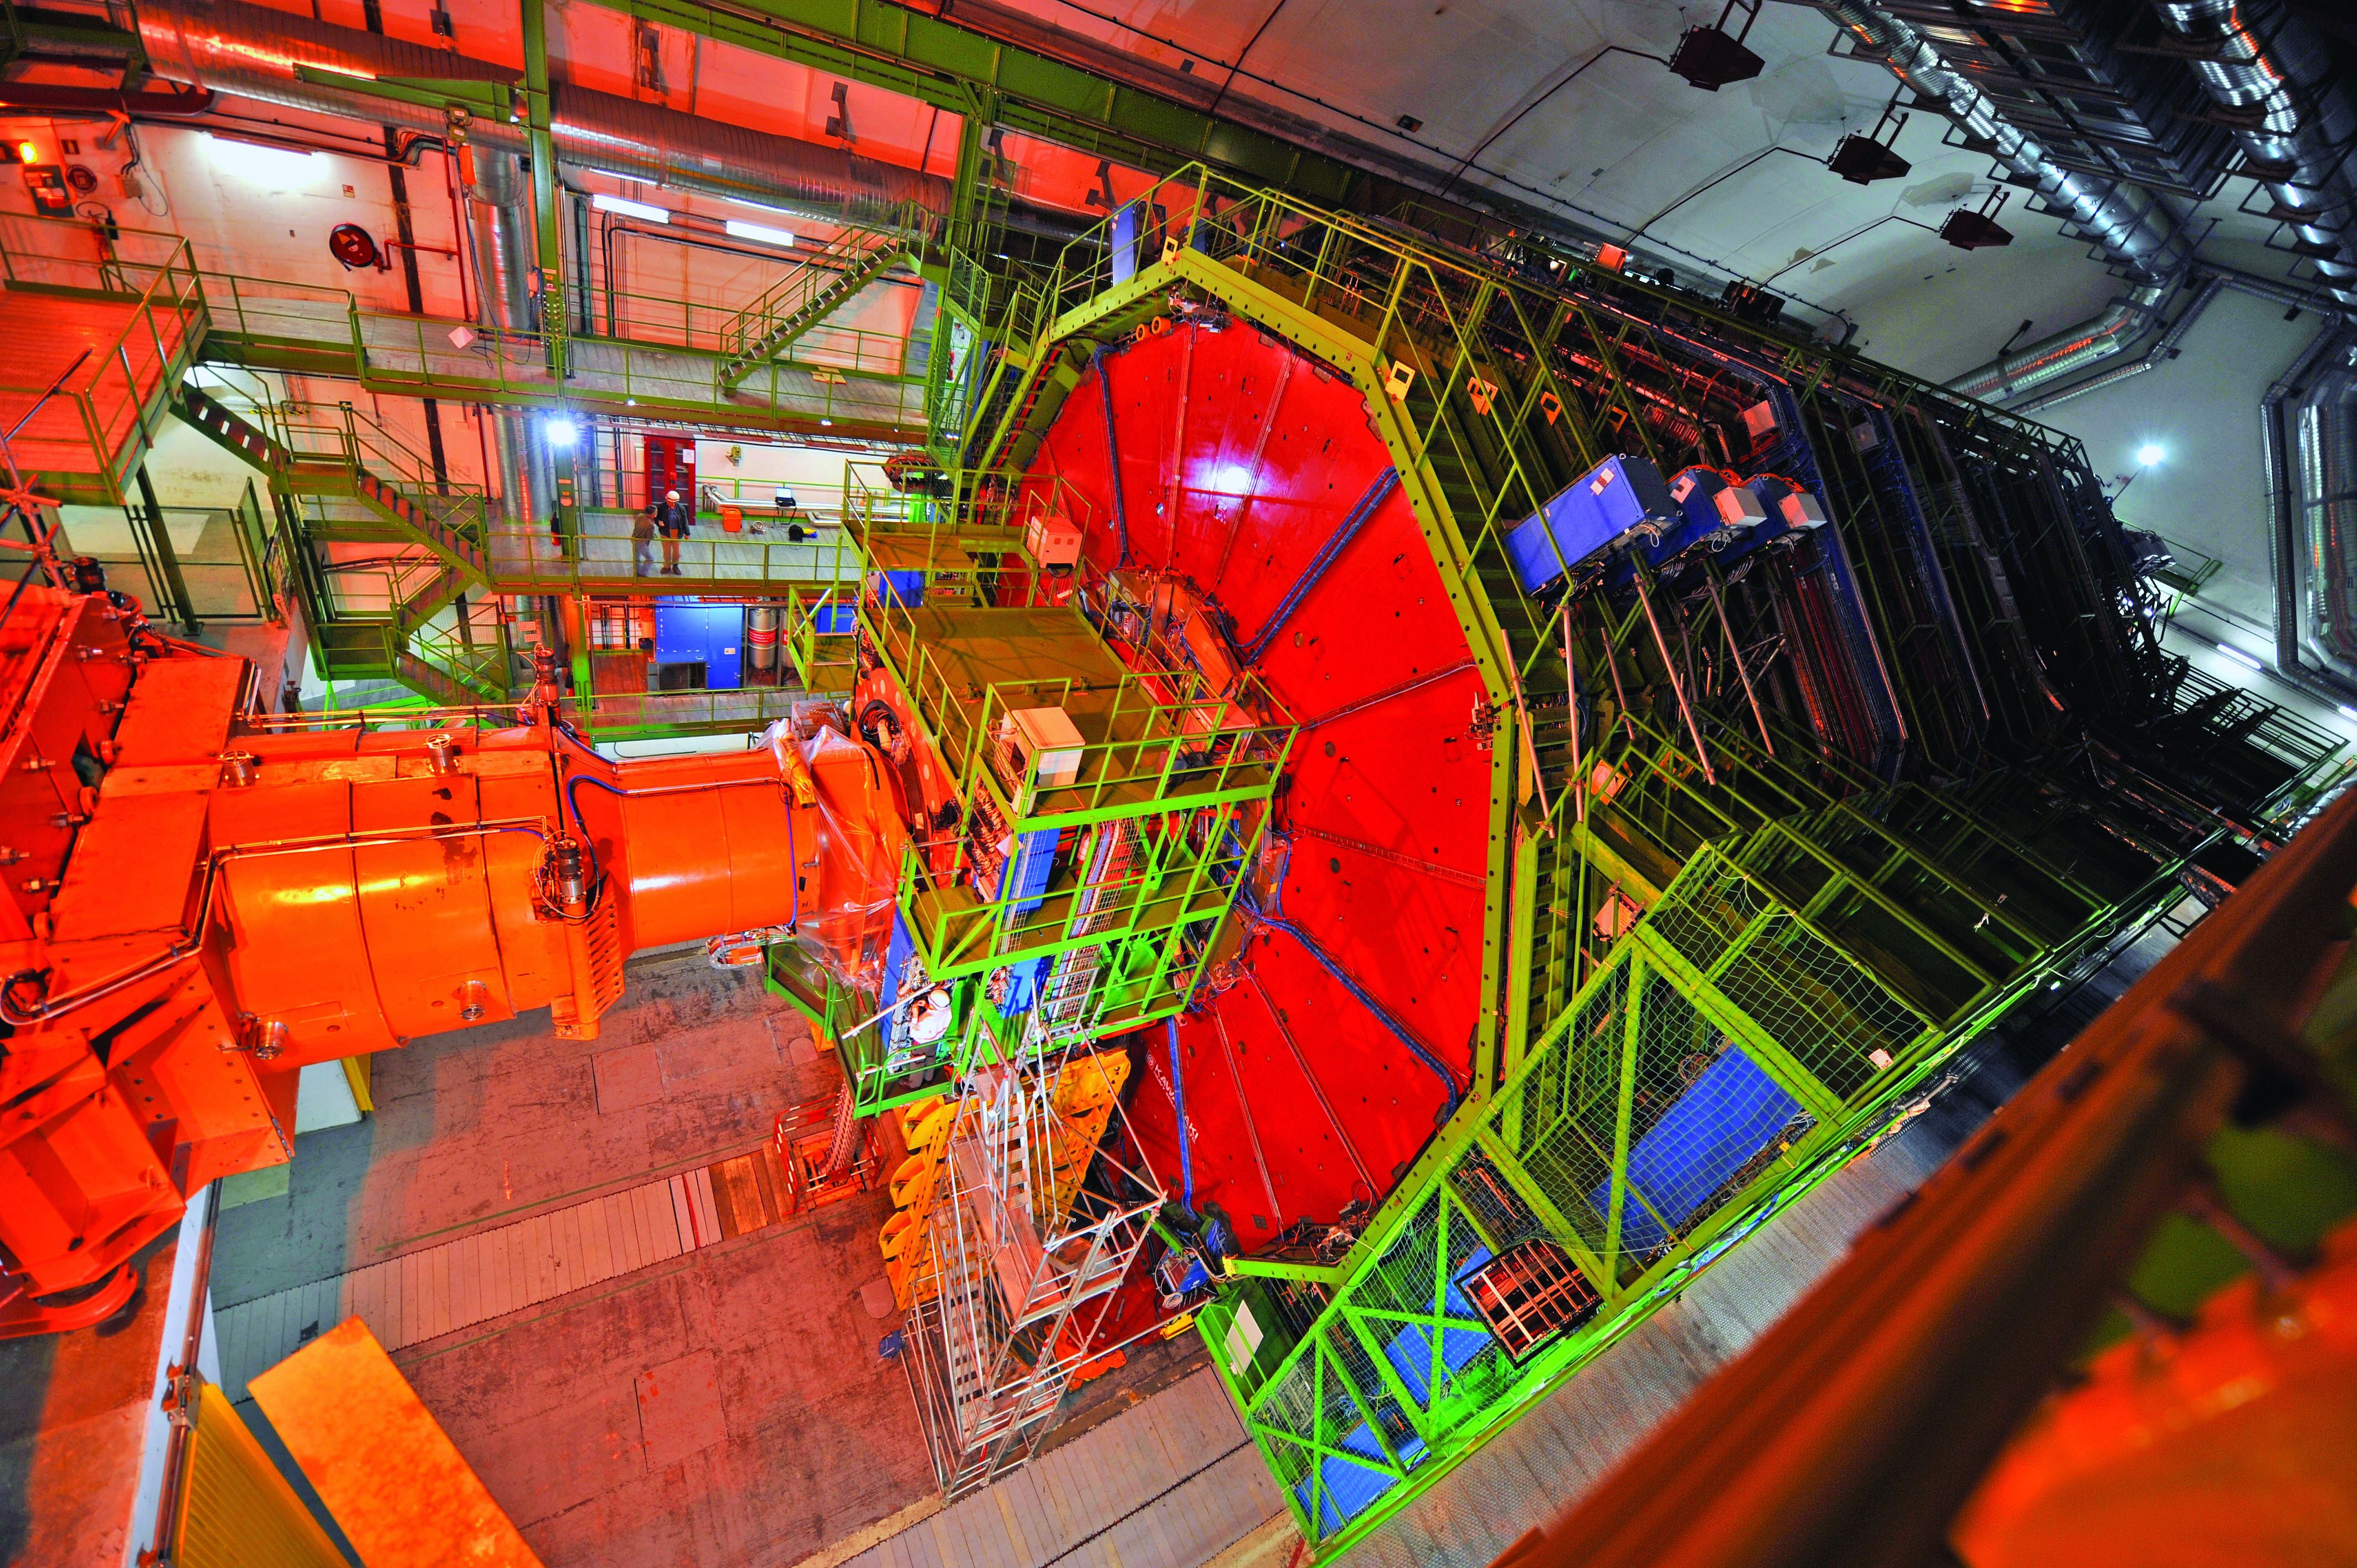
\includegraphics[width=0.492\textwidth,valign=c]{fig/cms/cms_picture3.jpg}}\quad
    \subfloat{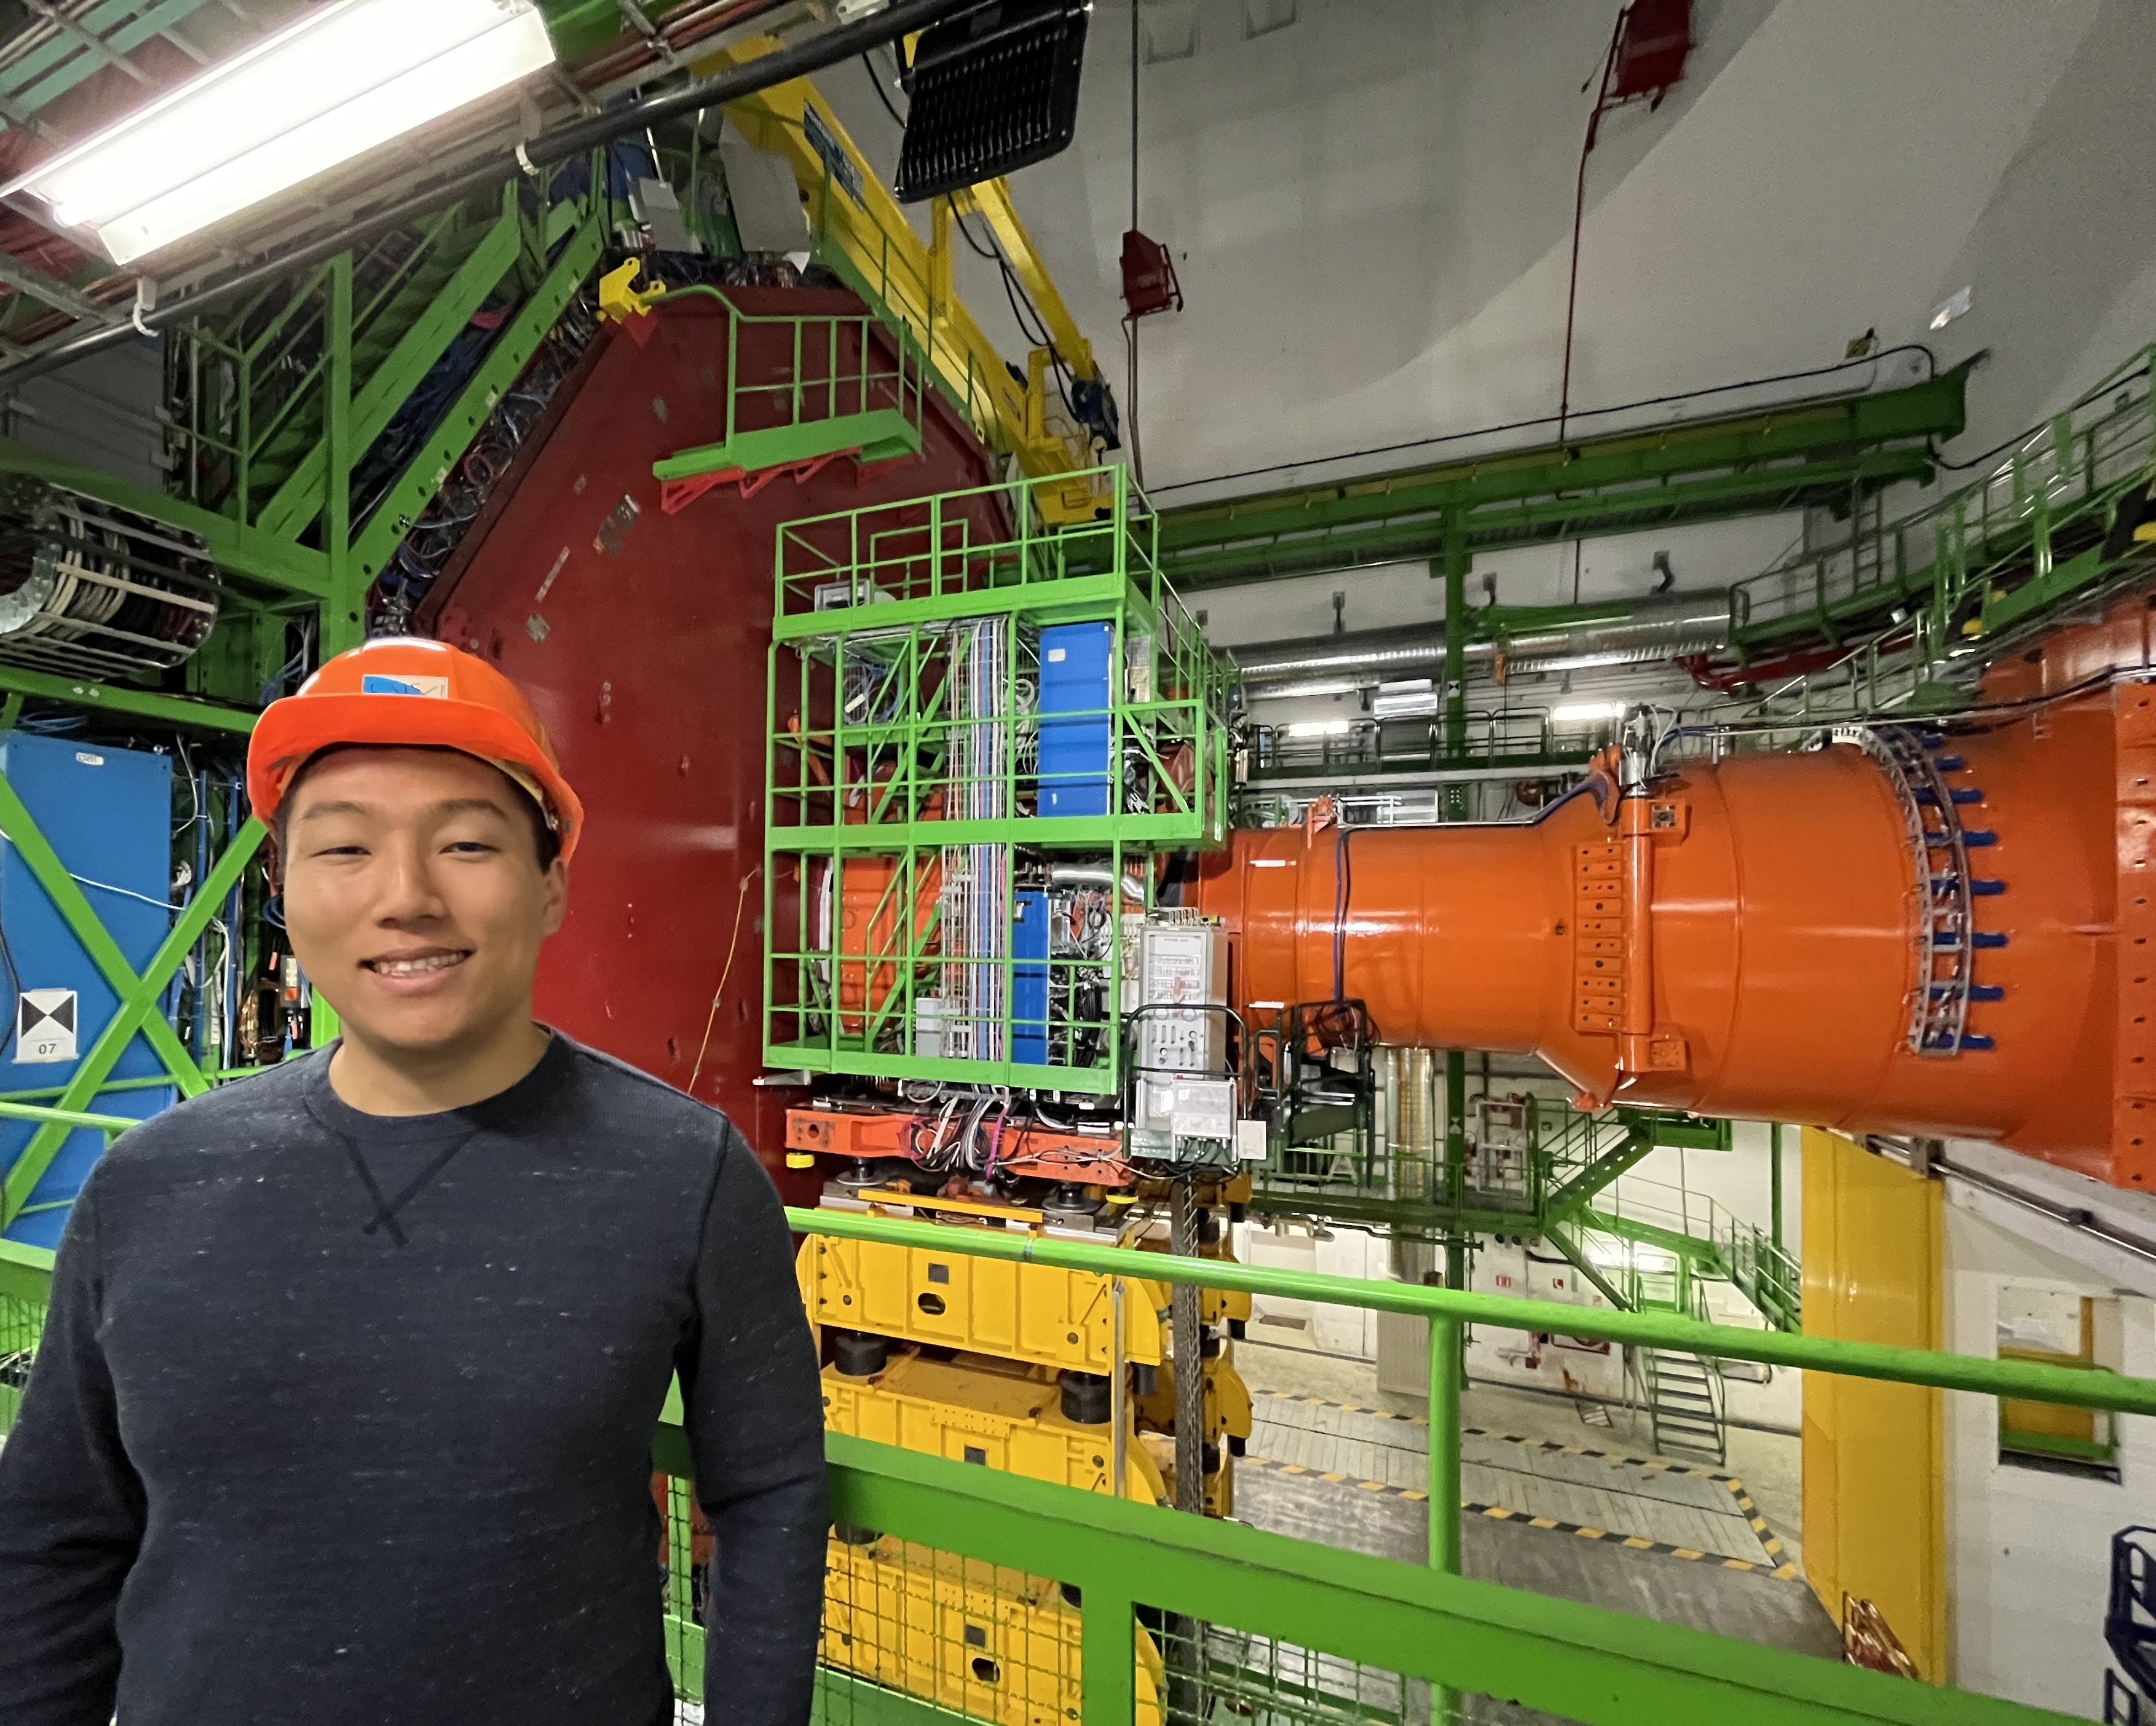
\includegraphics[width=0.408\textwidth,valign=c]{fig/cms/cms_jguiang.jpg}}
    \caption[CMS in the closed configuration, pictured from the top and side]{
        CMS in the closed configuration, pictured from the top (left), from Ref.~\cite{CMS:2009kms}, and side, with a physicist in the foreground for scale (right). 
    }
    \label{fig:cms_jguiang}
\end{figure}

\subsection{Overview}
The CMS Experiment is composed of subdetectors arranged in consecutive layers, where each layer interacts with or completely absorbs certain particles, producing an electric signal that can be used to measure some property of those particles. 
The innermost layer is the silicon tracker, which allows for the reconstruction of the trajectories of throughgoing charged particles (``tracks''). 
Next is the electromagnetic calorimeter (ECAL), which absorbs electrons and photons and records their individual energies. 
After the ECAL, there is the hadronic calorimeter (HCAL), which absorbs hadrons and records their individual energies. 
These first three layers---the tracker, ECAL, and HCAL---are surrounded by the eponymous CMS magnet, a superconducting solenoid that immerses the inner layers in an approximately uniform magnetic field that runs parallel to the beamline. 
This is critical: charged particles fly along curved trajectories in a magnetic field according to their charge and momentum, so those properties can be inferred from a high-quality measurement of each particle's trajectory. 
Finally, there are alternating layers of muon chambers, the other half of the experiment's namesake, and iron support structures. 
The former detects throughgoing muons, which pass through all of the inner layers mostly unperturbed, and measures an additional portion of their tracks.
However, the latter is equally important: the iron ``return yoke'' guides the magnetic field outside of the solenoid, absorbs stray particles that make it past the inner layers, and supports the immense weight of CMS itself. 
By combining information from all of these detectors, the exact identity of any individual particle can, in principle, be inferred based on which detectors registered a signal. 
Therefore, a full ``picture'' of each pp collision event is recorded by CMS for further study. 
The exact function of each subdetector layer described here is detailed below.

\subsection{Superconducting solenoid}
The curve of a track is critical, as it allows us to infer the charge and momentum of a particle. 
However, in a weak magnetic field, the particles produced at the LHC would have nearly straight tracks, due to the large pp collision energy. 
The magnetic field inside CMS must therefore be very large~\cite{CMSWebMagnet}. 
It should also be nearly uniform everywhere, in order to make the determination of each particle's charge and momentum as simple as possible. 
The CMS magnet must also be large in dimension, however, as it must surround the tracker, ECAL, and HCAL, since it would otherwise block outgoing particles. 

By winding copper wire into a helix and passing a current through it, we can generate a magnetic field whose strength is directly proportional to the current and number of turns of the wire, but inversely proportional to the length of the helix. 
Within the volume of the helix, the magnetic field will be almost uniformly oriented in a single direction, determined by the orientation of the helix and direction of the current (Fig.~\ref{fig:cms_magnet_ideal}). 
This is not true outside of the helix where the magnetic field lines curve in space. 

\begin{figure}[htb]
    \centering
    \subfloat[]{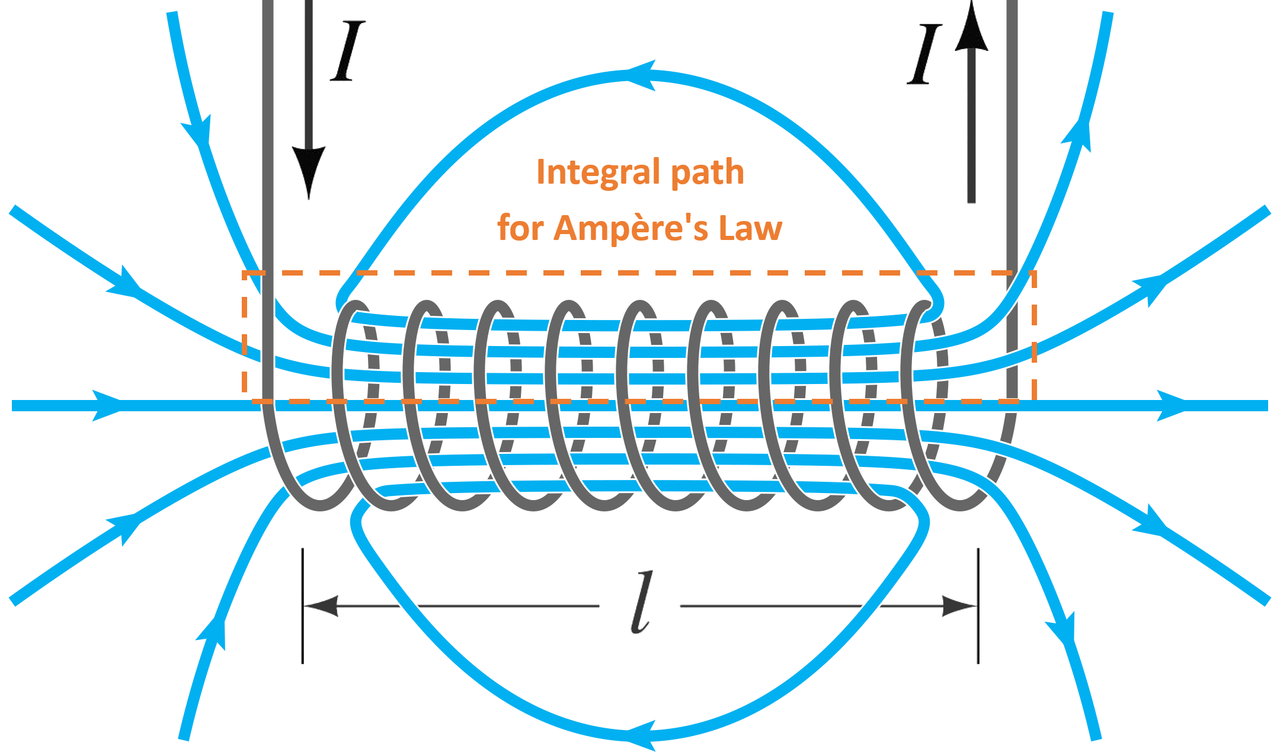
\includegraphics[width=0.4\textwidth,valign=c]{fig/cms/solenoid_ideal.png}\label{fig:cms_magnet_ideal}}\quad
    \subfloat[]{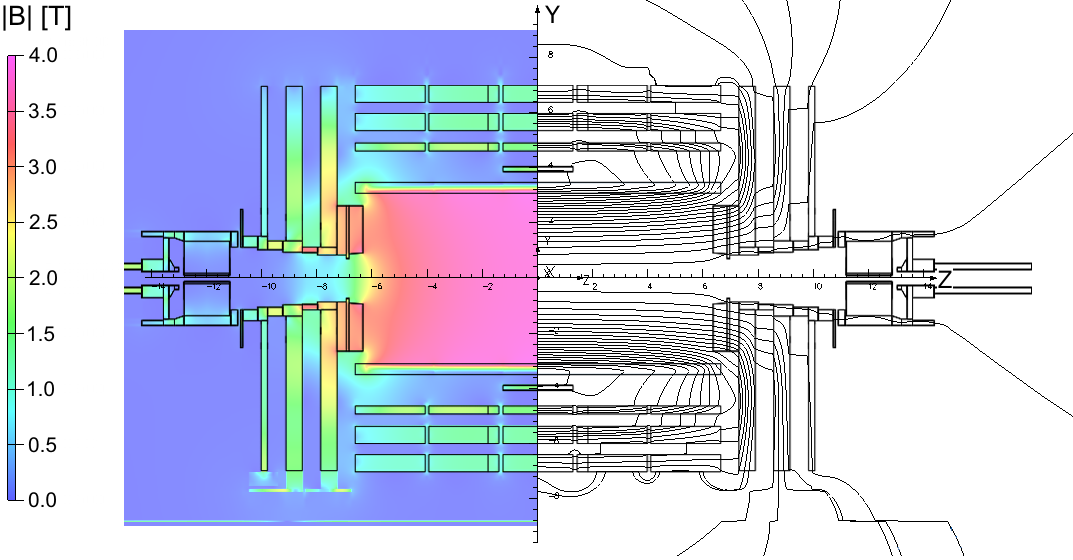
\includegraphics[width=0.5\textwidth,valign=c]{fig/cms/solenoid_field.png}\label{fig:cms_magnet_field}}
    \caption[The field lines of an ideal solenoid and those of the CMS magnet, from Ref.~\cite{CMS:2009moq}]{
        The field lines of an ideal solenoid (a), from Ref.~\cite{SolenoidFieldLines}, and those of the CMS magnet (b), from Ref.~\cite{CMS:2009moq}. 
        For the ideal solenoid, the magnetic field is described by a simple equation: $B = \mu_0\frac{NI}{l}$, where $\mu_0$ is the magnetic constant, $N$ is the number of turns, $I$ is the current, and $l$ is the length of the helix. 
    }
    \label{fig:cms_fields}
\end{figure}

The CMS magnet~\cite{CERN-LHCC-97-010} is a massive\footnotemark{} realization of a solenoid. 
\footnotetext{It was built offsite, however, so it needed to be designed to fit within 7 such that it could be wheeled through the streets in Cessy, France (under which CMS is situated)~\cite{CMSWebMagnet}.}
It is composed of over 2000 turns of Rutherford wire, which has a rectangular cross-section (Fig.~\ref{fig:cms_magnet}). 
In operation, it is cooled to superconducting temperatures (-268.5 \de{}C, or one degree warmer than outer space), such that a high current (20 kiloamperes\footnotemark{}) can be passed through the coil without violently destroying it. 
\footnotetext{For scale, this is 100\,000 times larger than the minimum fatal current for humans (100--200 milliamperes)~\cite{10.1093/ptj/46.9.968}.}
This configuration allows the CMS magnet to produce a mostly uniform magnetic field of 4 T inside the solenoid volume. 
That is 2--4 times larger than an MRI, which are typically 0.5--1.5 T~\cite{Berger2002-gs}, within a volume that is 1000 times larger. 
We must also, however, have a fairly uniform magnetic field outside of the solenoid in order to maintain good momentum resolution for muons. 
To achieve this, the iron support structures that hold CMS together are also designed to guide the magnetic field lines (Fig.~\ref{fig:cms_magnet_field}). 
Inside the iron, the magnetic field runs almost uniformly parallel to the field inside the solenoid, but in the opposite direction---this gives muon tracks a characteristic S-shape in the transverse plane (Fig.~\ref{fig:cms_muon_diagram}). 

\begin{figure}[htb]
    \centering
    \subfloat{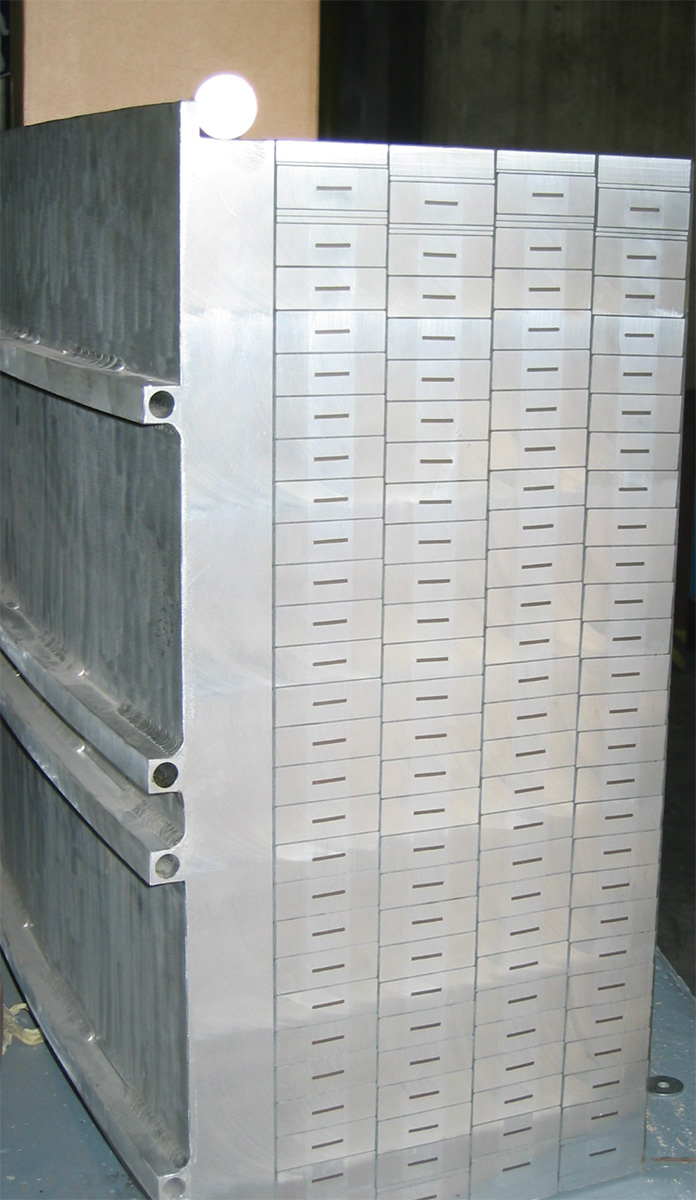
\includegraphics[width=0.3\textwidth,valign=c]{fig/cms/solenoid_wedge.jpg}}\quad
    \subfloat{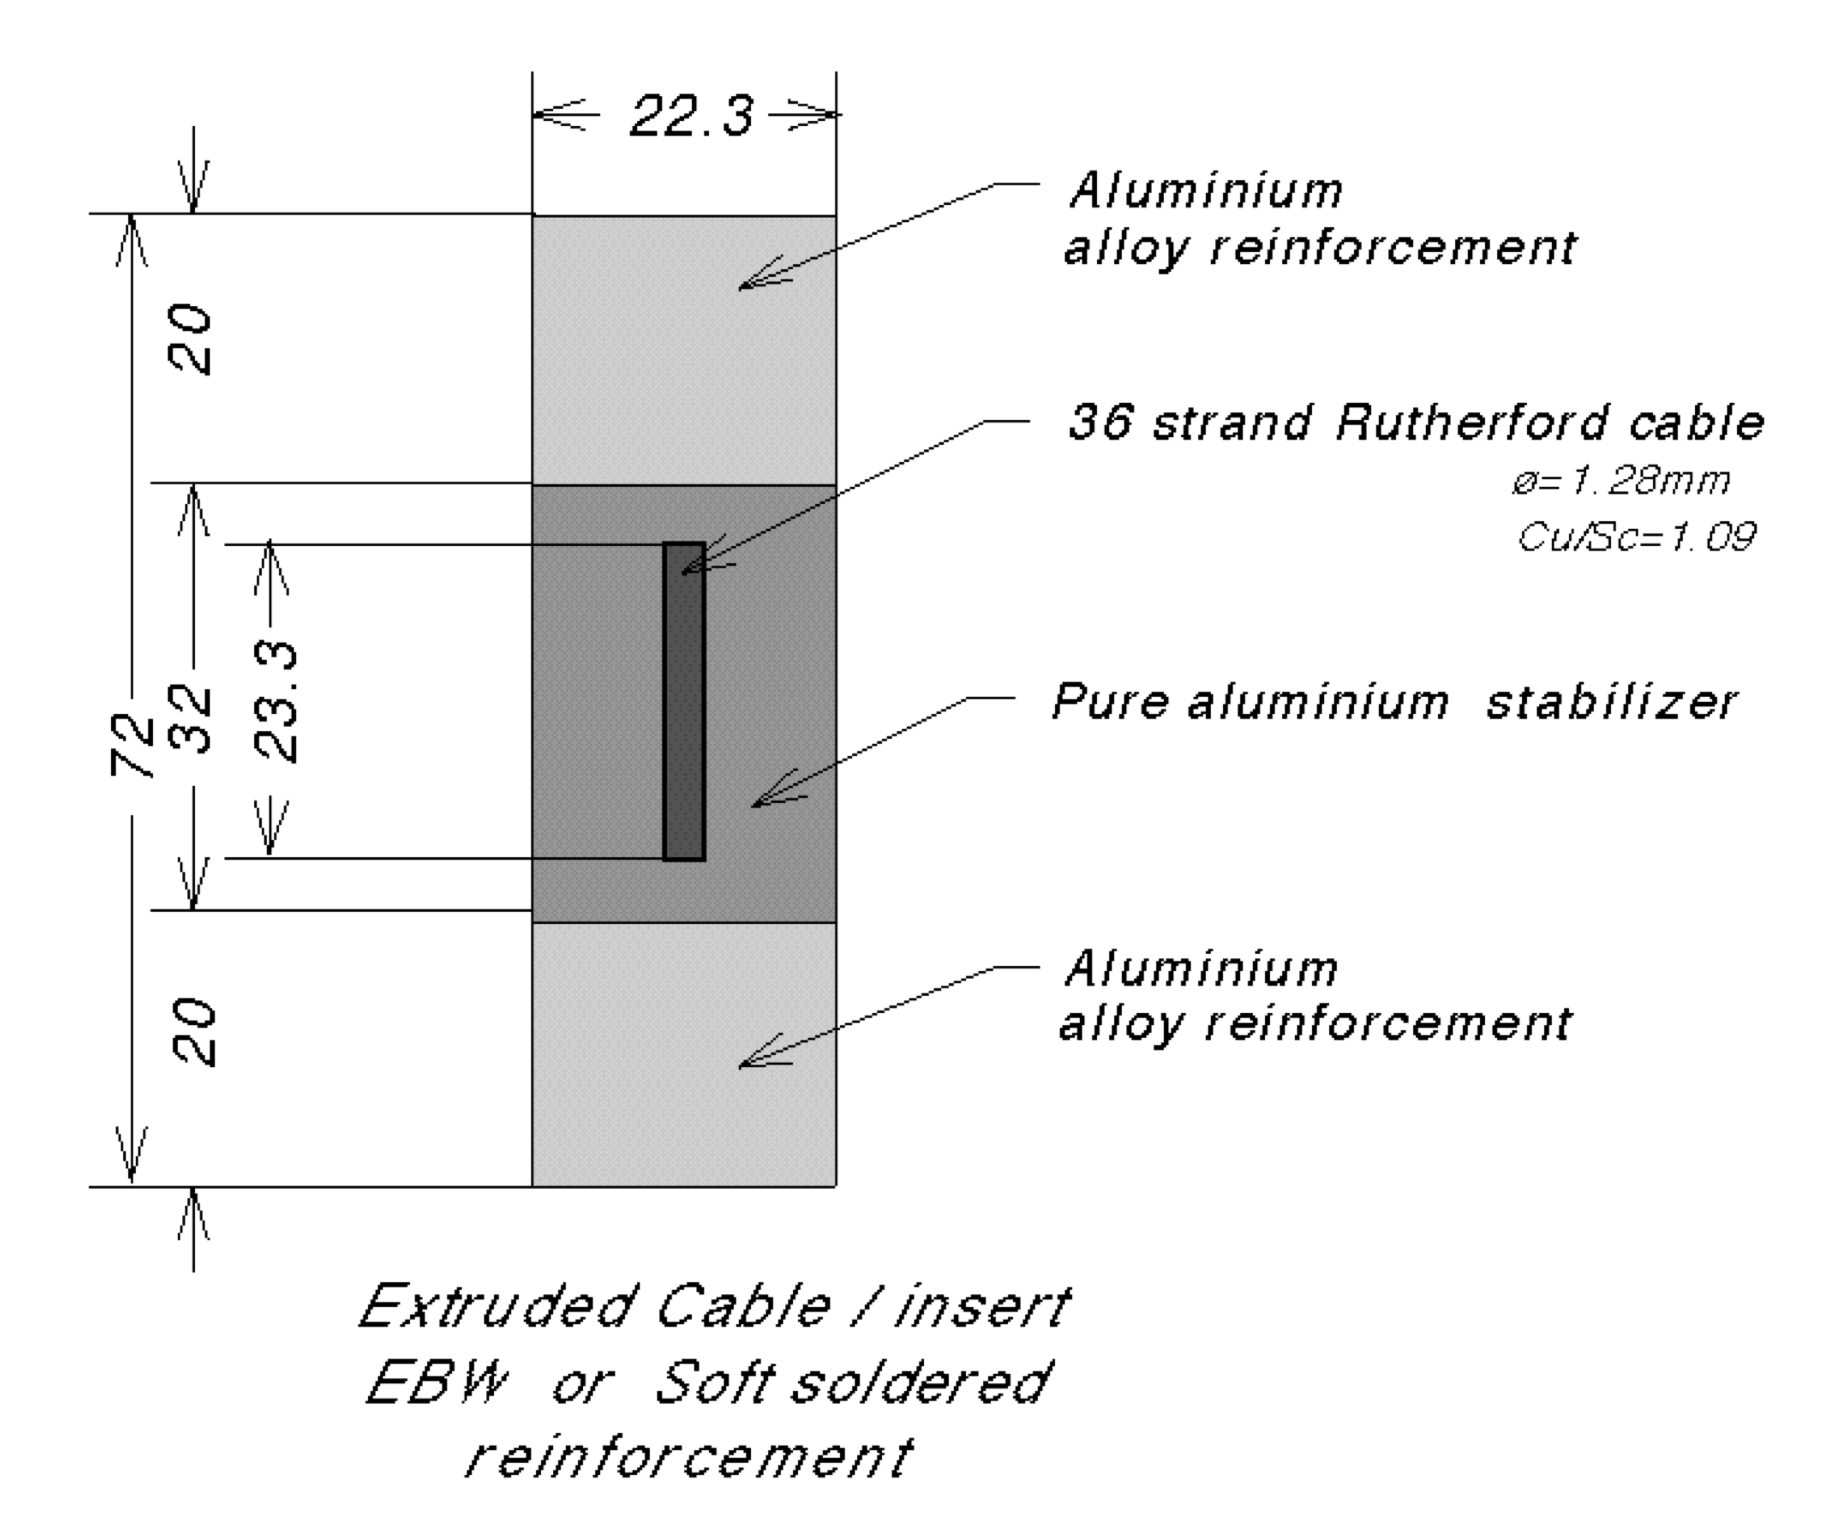
\includegraphics[width=0.6\textwidth,valign=c]{fig/cms/solenoid_cable.png}}
    \caption[A photograph of a section of the CMS magnet, from Ref.~\cite{CourierSolenoid}, and a diagram of a single winding, from Ref.~\cite{CERN-LHCC-97-010}]{
        A photograph of a section of the CMS magnet, from Ref.~\cite{CourierSolenoid}, showing the cross-section of the solenoid winding (left), and a diagram of a single winding, from Ref.~\cite{CERN-LHCC-97-010} (right). 
    }
    \label{fig:cms_magnet}
\end{figure}

\subsection{Silicon tracker}
In order to reconstruct the track of any particle, we need its position at multiple points in time. 
A tracker records these positions. 
Mechanically, this can be done in a variety of ways. 
Some of the earliest particle physics experiments used bubble chambers, a device that maintains (for a brief instance) a volume of superheated liquid immersed in a magnetic field in which throughgoing charged particles leave helical trails of bubbles. 
Photographs of these trails were used to infer the identities of each particle. 
Still others used even more exotic non-electric solutions, like the OPERA Experiment, which used enormous layers of nuclear emulsion film (modified photography film) in which throughgoing particles would leave tiny black dots after the film was developed\footnotemark{}~\cite{Acquafredda:2009zz}---the experiment used over 100\,000 m$^2$ of emulsion film in total. 
\footnotetext{Developing the film was quite an operation, and a large robotic arm was used to remove and replace the layers.}

The leading challenge in designing the CMS tracker was the unprecedented level of radiation, due to the high frequency of pp collisions, which each produce many thousands of particles. 
Existing tracker designs, like the CDF Experiment's beautiful gas-and-wire tracker~\cite{CDF:2003xbh}, would quickly break down\footnotemark{} in this kind of environment.
\footnotetext{In fact, the tracker section was left blank in the first CMS design document, since there were no known solutions at the time~\cite{CMSWebTracker}.}
Thankfully, advances in radiation-hard electronics yielded a new solution. 
In particular, a silicon-based tracking module was devised. 
When charged particles pass through the module, they liberate electrons from the silicon atoms. 
These electrons are collected on one of many small readout plates, which results in a localized electric signal called a ``hit,'' giving excellent spatial resolution. 

The CMS tracker is composed of multiple layers of silicon tracker modules (Fig.~\ref{fig:cms_tracker_layout}), such that each throughgoing particle leaves multiple hits that can then be used to reconstruct its track. 
The layers are grouped into different sections according to their proximity to the beamline and their geometry. 
The innermost layers comprise the ``inner tracker'' (Fig.~\ref{fig:cms_tracker_inner}). 
In these layers, pixel modules are used because they have superior spatial resolution, allowing us to measure the first portion of each track precisely. 
The outermost layers comprise the ``outer tracker'' (Fig.~\ref{fig:cms_tracker_outer}). 
These layers use strip modules, which have worse spatial resolution than the pixel modules, but are easier to produce. 

\begin{figure}[htb]
    \centering
    \subfloat[]{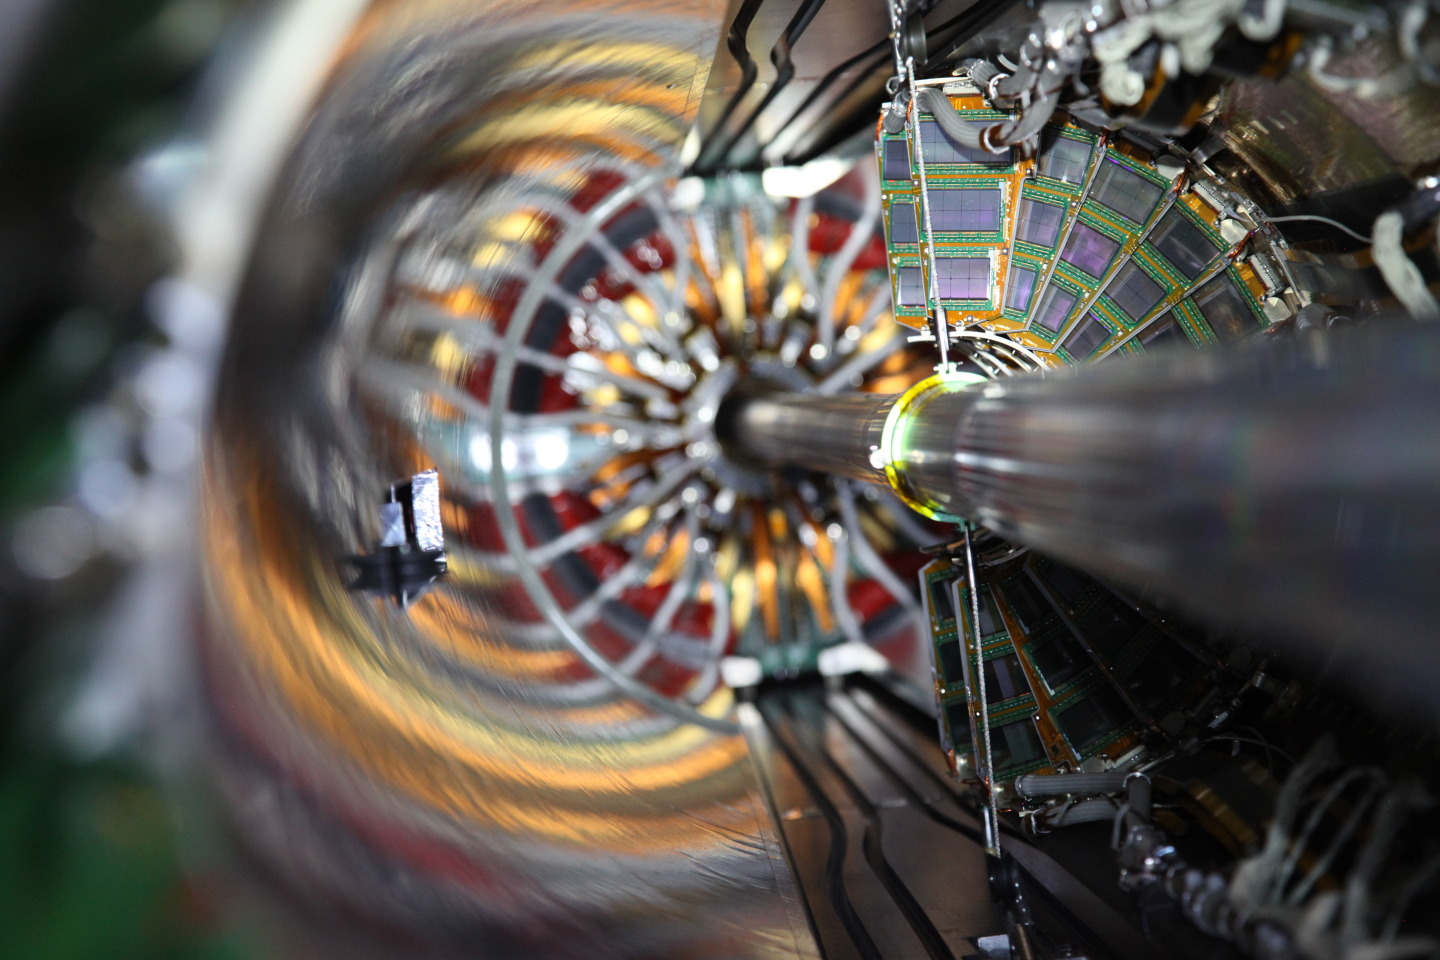
\includegraphics[width=0.45\textwidth,valign=c]{fig/cms/tracker_pixels.jpg}\label{fig:cms_tracker_inner}}\quad
    \subfloat[]{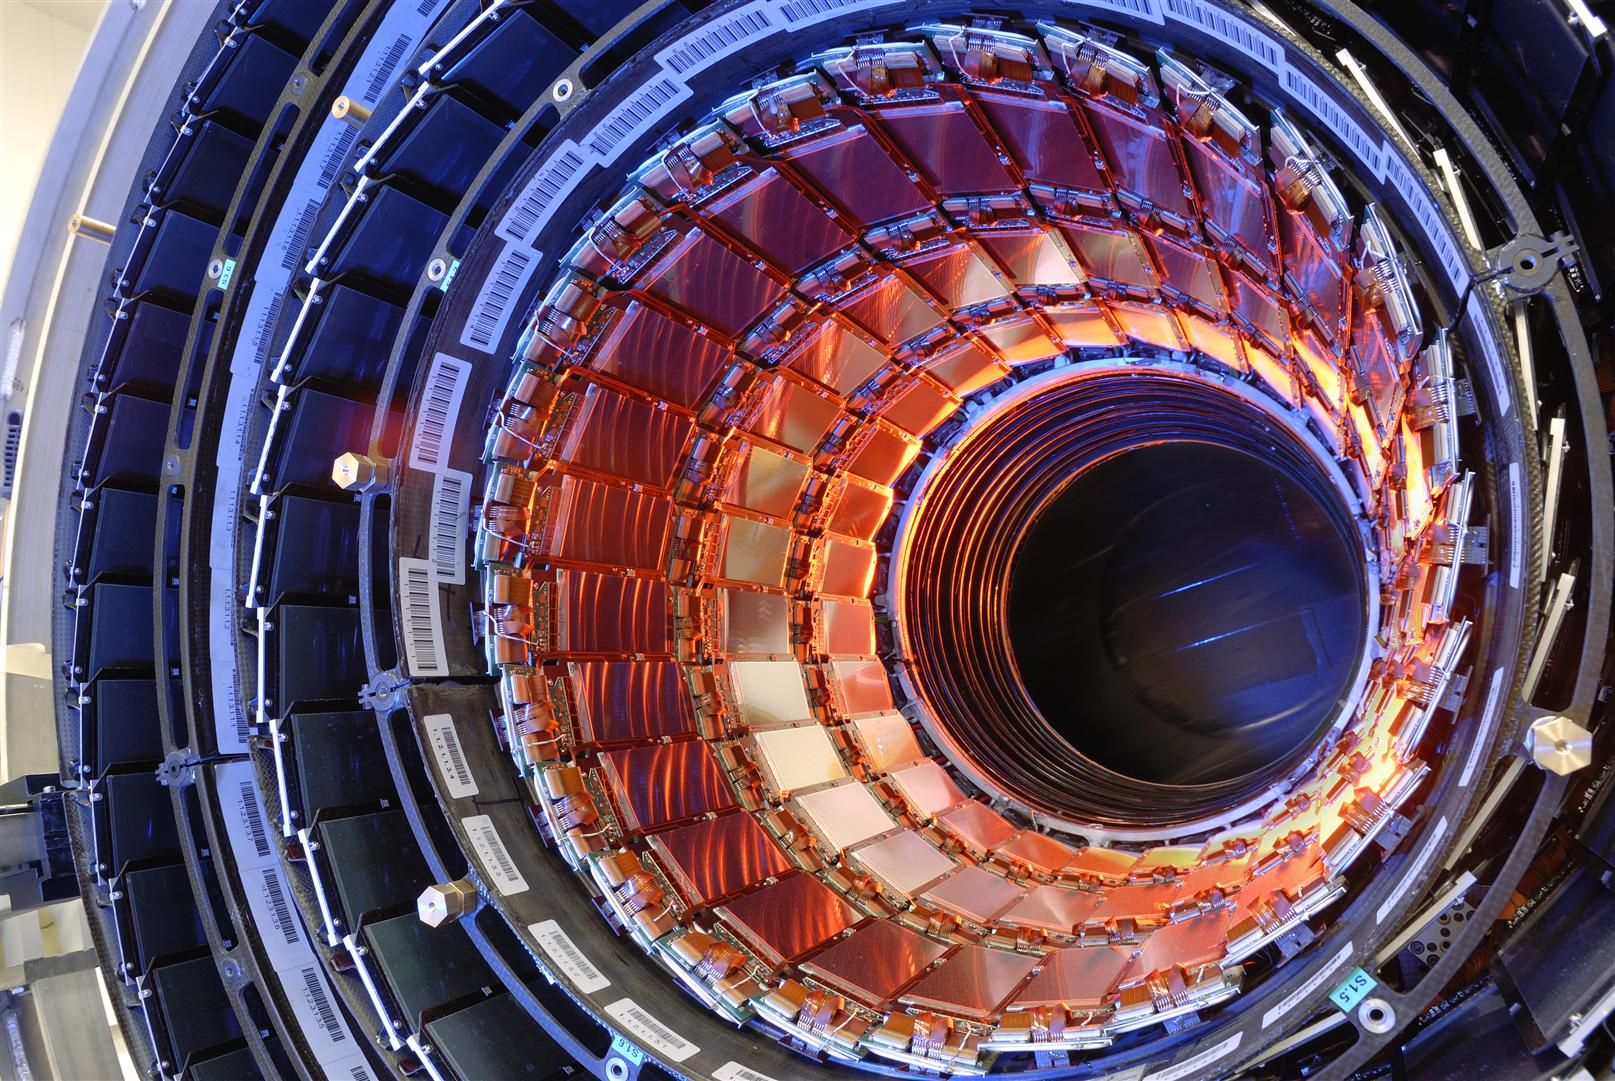
\includegraphics[width=0.45\textwidth,valign=c]{fig/cms/tracker_rainbow.jpg}\label{fig:cms_tracker_outer}}
    \caption[A photograph of the CMS silicon tracker inner forward pixel modules, from Ref.~\cite{Hoch:2017264}, and the outer barrel layers with a physicist in the background for scale, from Ref.~\cite{Maximilien:995912}]{
        A photograph of the CMS silicon tracker inner forward pixel modules (left), from Ref.~\cite{Hoch:2017264}, and the outer barrel layers with a physicist in the background for scale (right), from Ref.~\cite{Maximilien:995912}. 
    }
    \label{fig:cms_tracker_pictures}
\end{figure}

\begin{figure}[htb]
    \centering
    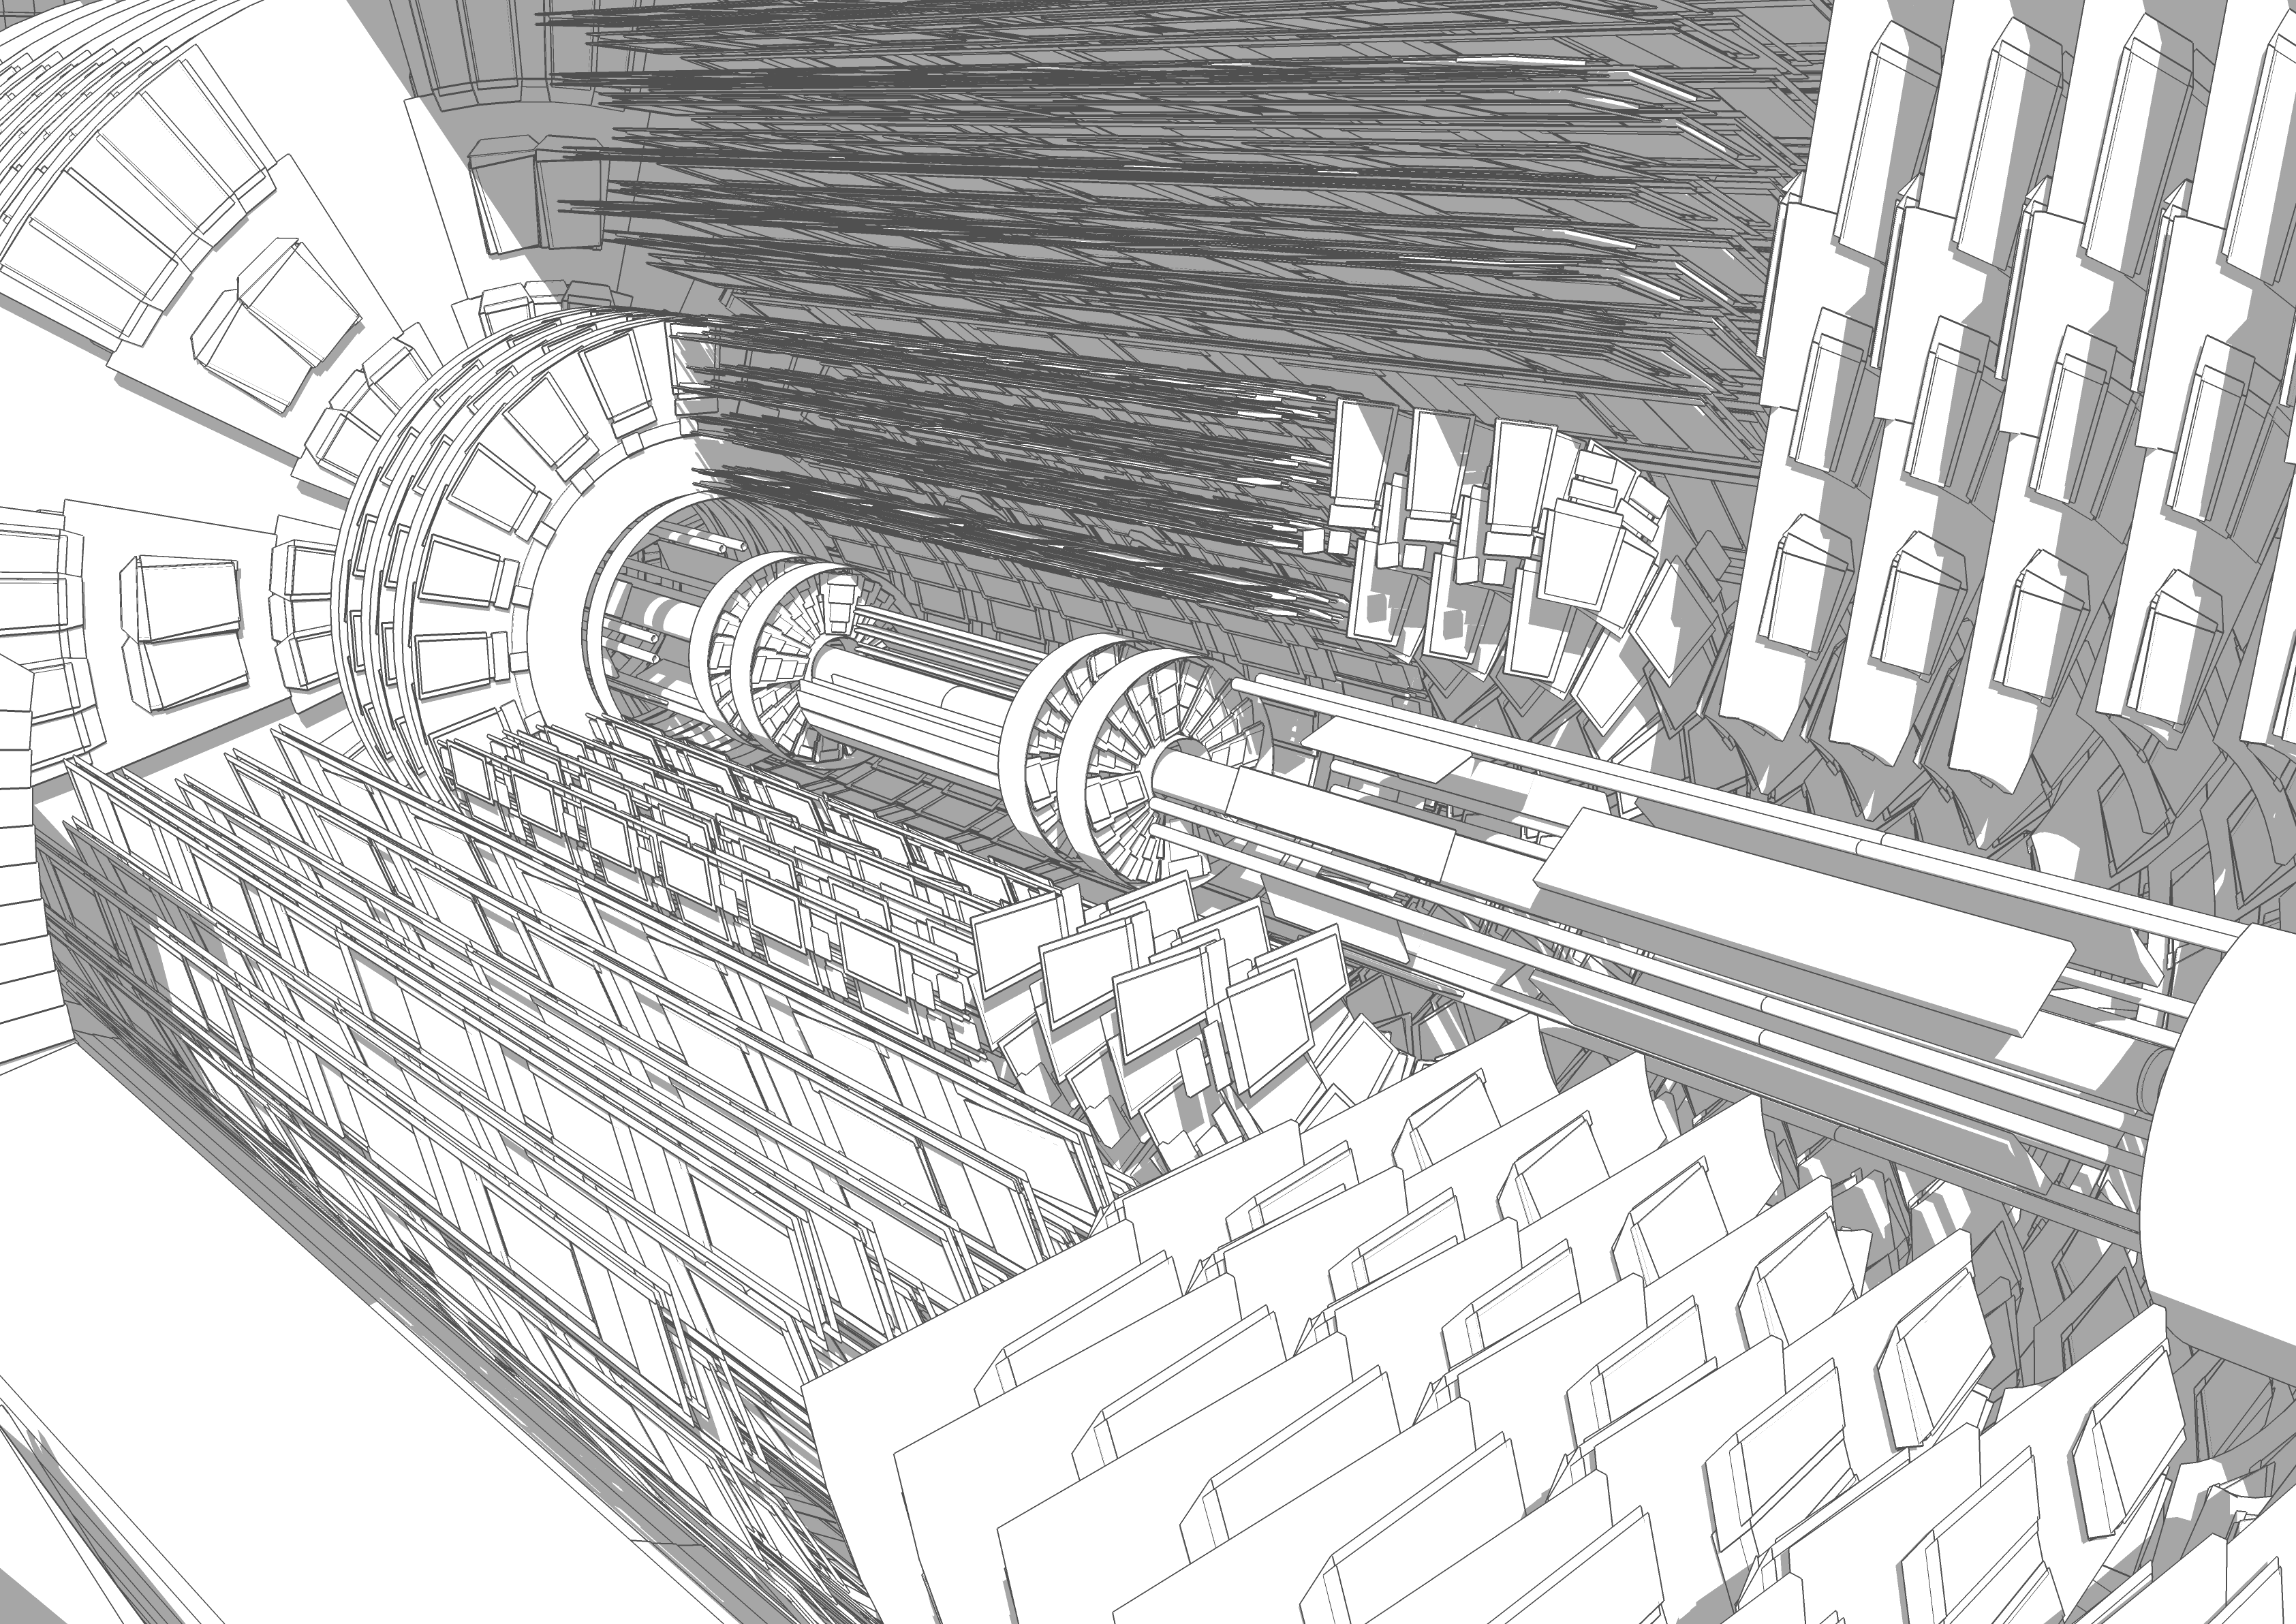
\includegraphics[width=0.9\textwidth,valign=c]{fig/cms/tracker_detailed.png}
    \caption{
        A detailed cutaway diagram of the CMS Phase-1 tracker from Ref.~\cite{Sakuma:2630160}. 
    }
    \label{fig:cms_tracker_layout}
\end{figure}

\subsection{Electromagnetic calorimeter}
The ECAL (Fig.~\ref{fig:cms_ecal_install}) consists of nearly 80\,000 lead tungstate (PbWO$_4$) crystals\footnotemark{} (Fig.~\ref{fig:cms_ecal_crystal})~\cite{CMSWebECAL}. 
\footnotetext{These crystals were grown in manufacturing plants in Russia and China and took roughly a decade to produce~\cite{CMSWebECAL}.}
When an electron or photon passes through one of these crystals, they interact through the electromagnetic force with the atoms in the crystal lattice, producing a shower of photons. 
This process is called ``scintillation'' and the amount of light produced from one of these interactions is proportional to the energy of the impinging particle. 
Each PbWO$_4$ crystal is glued to a photodetector that collects the scintillation light by the attached crystal and outputs an electric signal proportional to the amount of light collected. 
This signal can then be used to measure the energy of electrons and photons. 

The probability of material interactions occurring as well as the shape of the shower varies amongst scintillating materials. 
Ultimately, PbWO$_4$ was selected for its short radiation length and small Moli\`ere radius~\cite{CERN-LHCC-97-033}, corresponding to a high probability of interactions and showers localized mostly to a single crystal, respectively. 
The former property is most obviously useful: a high probability of scintillation means electrons and photons are more efficiently collected by the ECAL. 
The latter property, however, is also vital: localized showers are less likely to overlap, so individual particles can be resolved. 

\begin{figure}[htb]
    \centering
    \subfloat[]{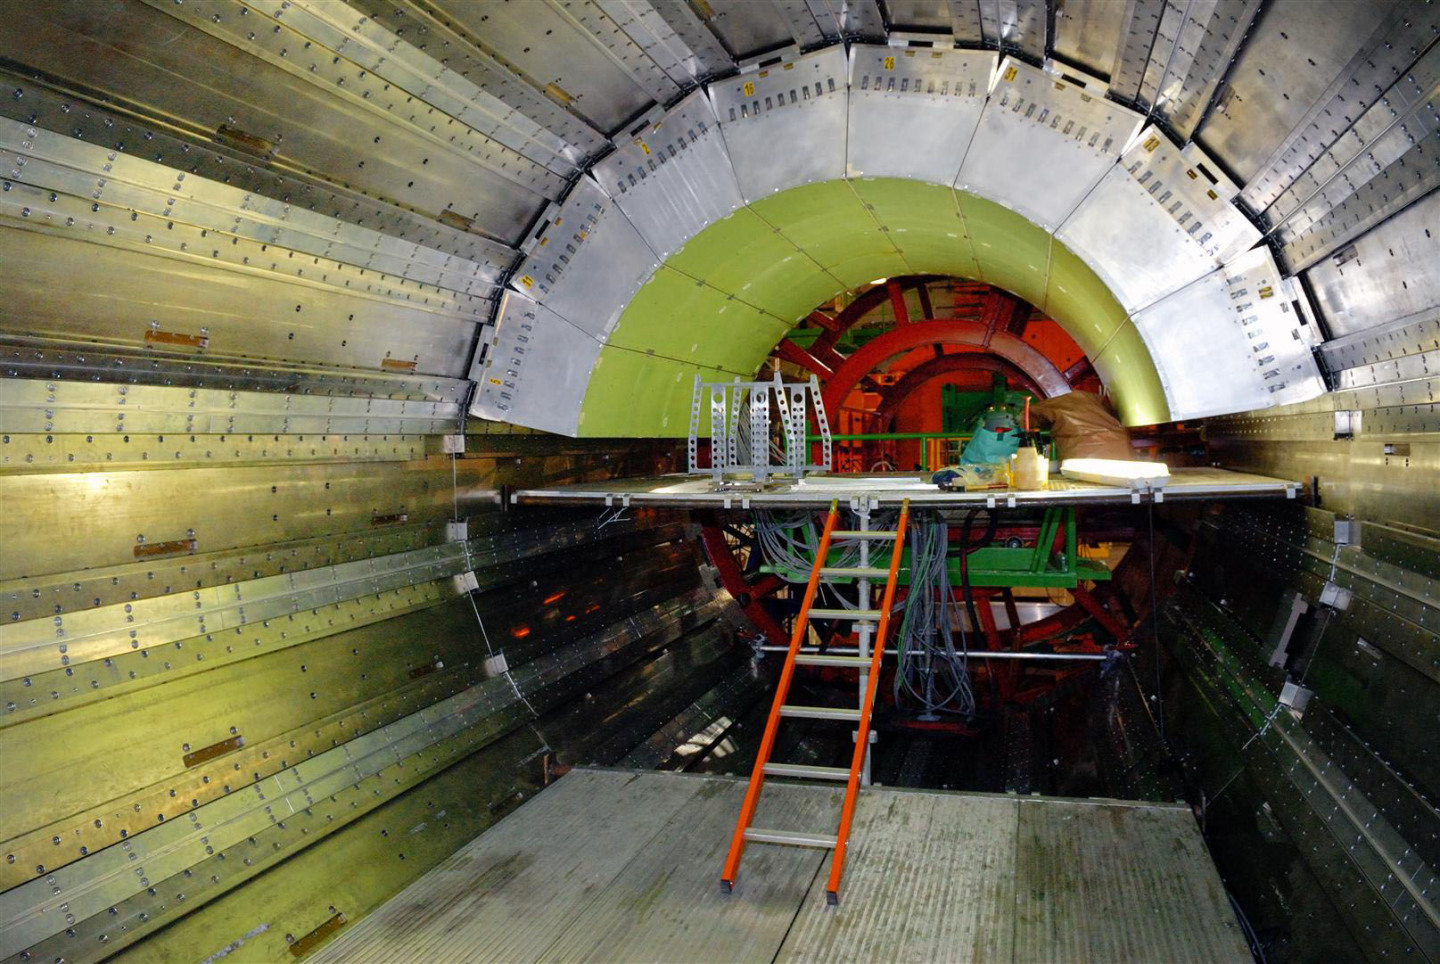
\includegraphics[width=0.45\textwidth,valign=c]{fig/cms/ecal_install.jpg}\label{fig:cms_ecal_install}}\quad
    \subfloat[]{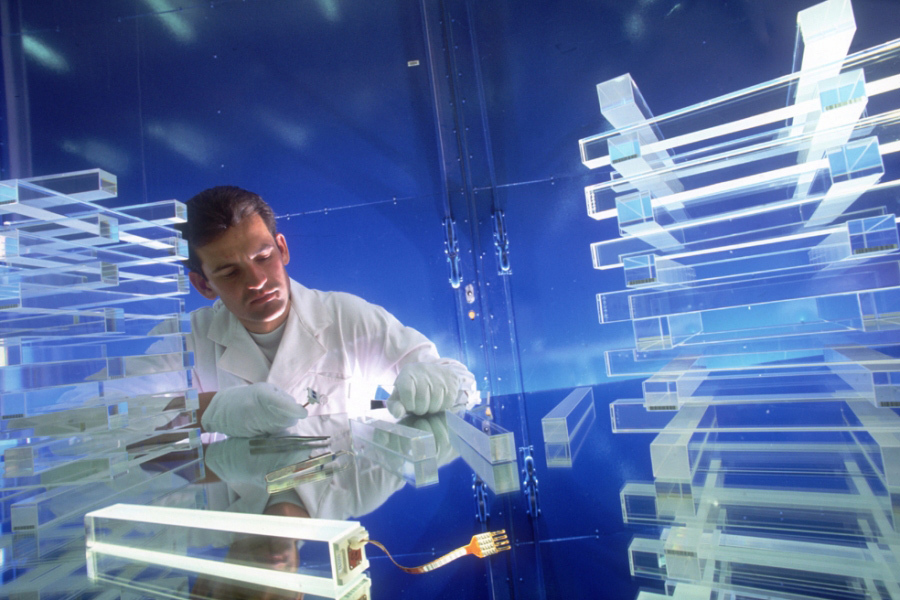
\includegraphics[width=0.45\textwidth,valign=c]{fig/cms/ecal_crystal.jpg}\label{fig:cms_ecal_crystal}}
    \caption[A photograph of the CMS electromagnetic calorimeter (ECAL) after half of the modules had been installed, and a physicist posed with the lead tungstate scintillator crystals used in the ECAL]{
        A photograph of the CMS electromagnetic calorimeter (ECAL) after half of the modules had been installed (left), and a physicist posed with the lead tungstate scintillator crystals used in the ECAL (right). 
        Both photographs are from Ref.~\cite{Brice:1431477}.
    }
    \label{fig:cms_ecal}
\end{figure}

\subsection{Hadronic calorimeter}
The HCAL (Fig.~\ref{fig:cms_hcal_removed}) is composed of interwoven layers of solid brass or steel plates and plastic scintillator tiles~\cite{CERN-LHCC-97-031}. 
When a hadron interacts with one of the brass and steel ``absorber'' layers, a shower of secondary particles are created. 
The secondary particles pass through the next scintillator layer, creating scintillation light, then proceed to the next absorber layer. 
In this way, large cascading showers of secondary particles are produced according to the energy of the impinging particle, where each scintillator layer gives some measurement, or ``sample,'' of the original particle's energy. 

This kind of calorimeter, which has alternating absorber and scintillator layers, is called a ``sampling'' calorimeter as opposed to a ``homogeneous'' calorimeter, wherein a single medium is used to both create the shower and measure the energy. 
Sampling calorimeters are typically less costly and give some information on the shape of the shower, whereas homogeneous calorimeters have superior energy resolution. 
However, a homogeneous hadronic calorimeter would need to be infeasibly large in order to fully contain a hadronic shower~\cite{KolanoskiWermesDetectors}. 
It is particularly critical that the HCAL be compact for CMS, as every increase in size of the inner layers results in large increases in volume of the solenoid and muon chambers, resulting in enormous increases in energy and material costs. 
Due to these space constraints, an additional layer of the HCAL needed to be placed outside of the magnet in order to measure, and absorb, anything that made it past the bulk of the HCAL. 
In fact, the HCAL was already projected to be too costly due to the sheer amount of high-quality brass needed to create the absorber plates. 
To save on costs, the Russian Navy was convinced to recycle over one million World War II artillery shells (Fig.~\ref{fig:cms_hcal_russian}), which were designed to withstand a large amount of stress (read: explosions) and years at sea, for the cause~\cite{CMSWebHCAL}. 

\begin{figure}[htb]
    \centering
    \subfloat{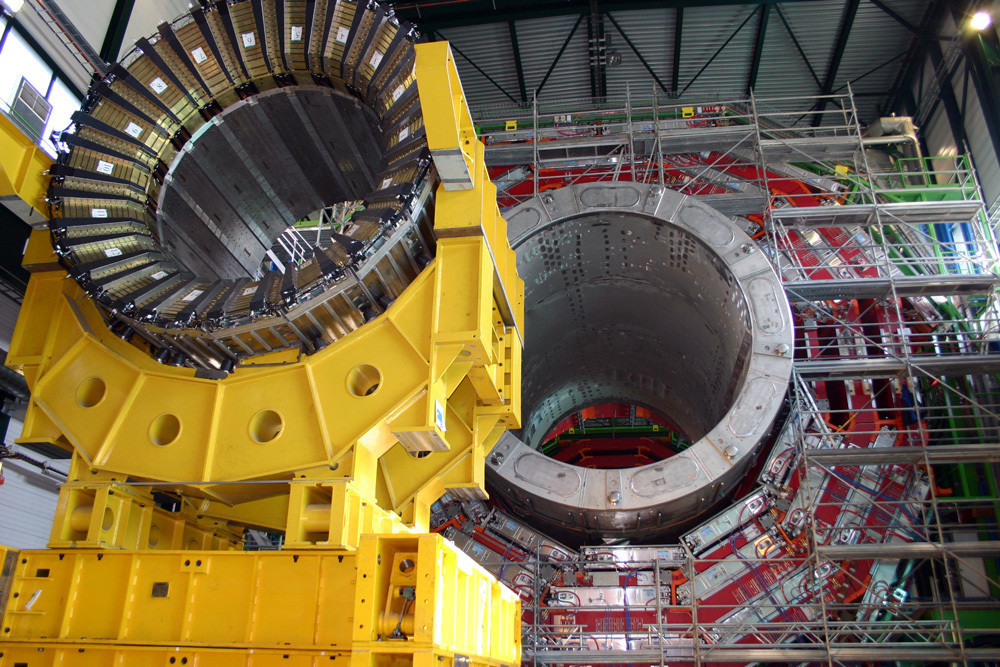
\includegraphics[width=0.45\textwidth,valign=c]{fig/cms/hcal_removed.jpg}\label{fig:cms_hcal_removed}}\quad
    \subfloat{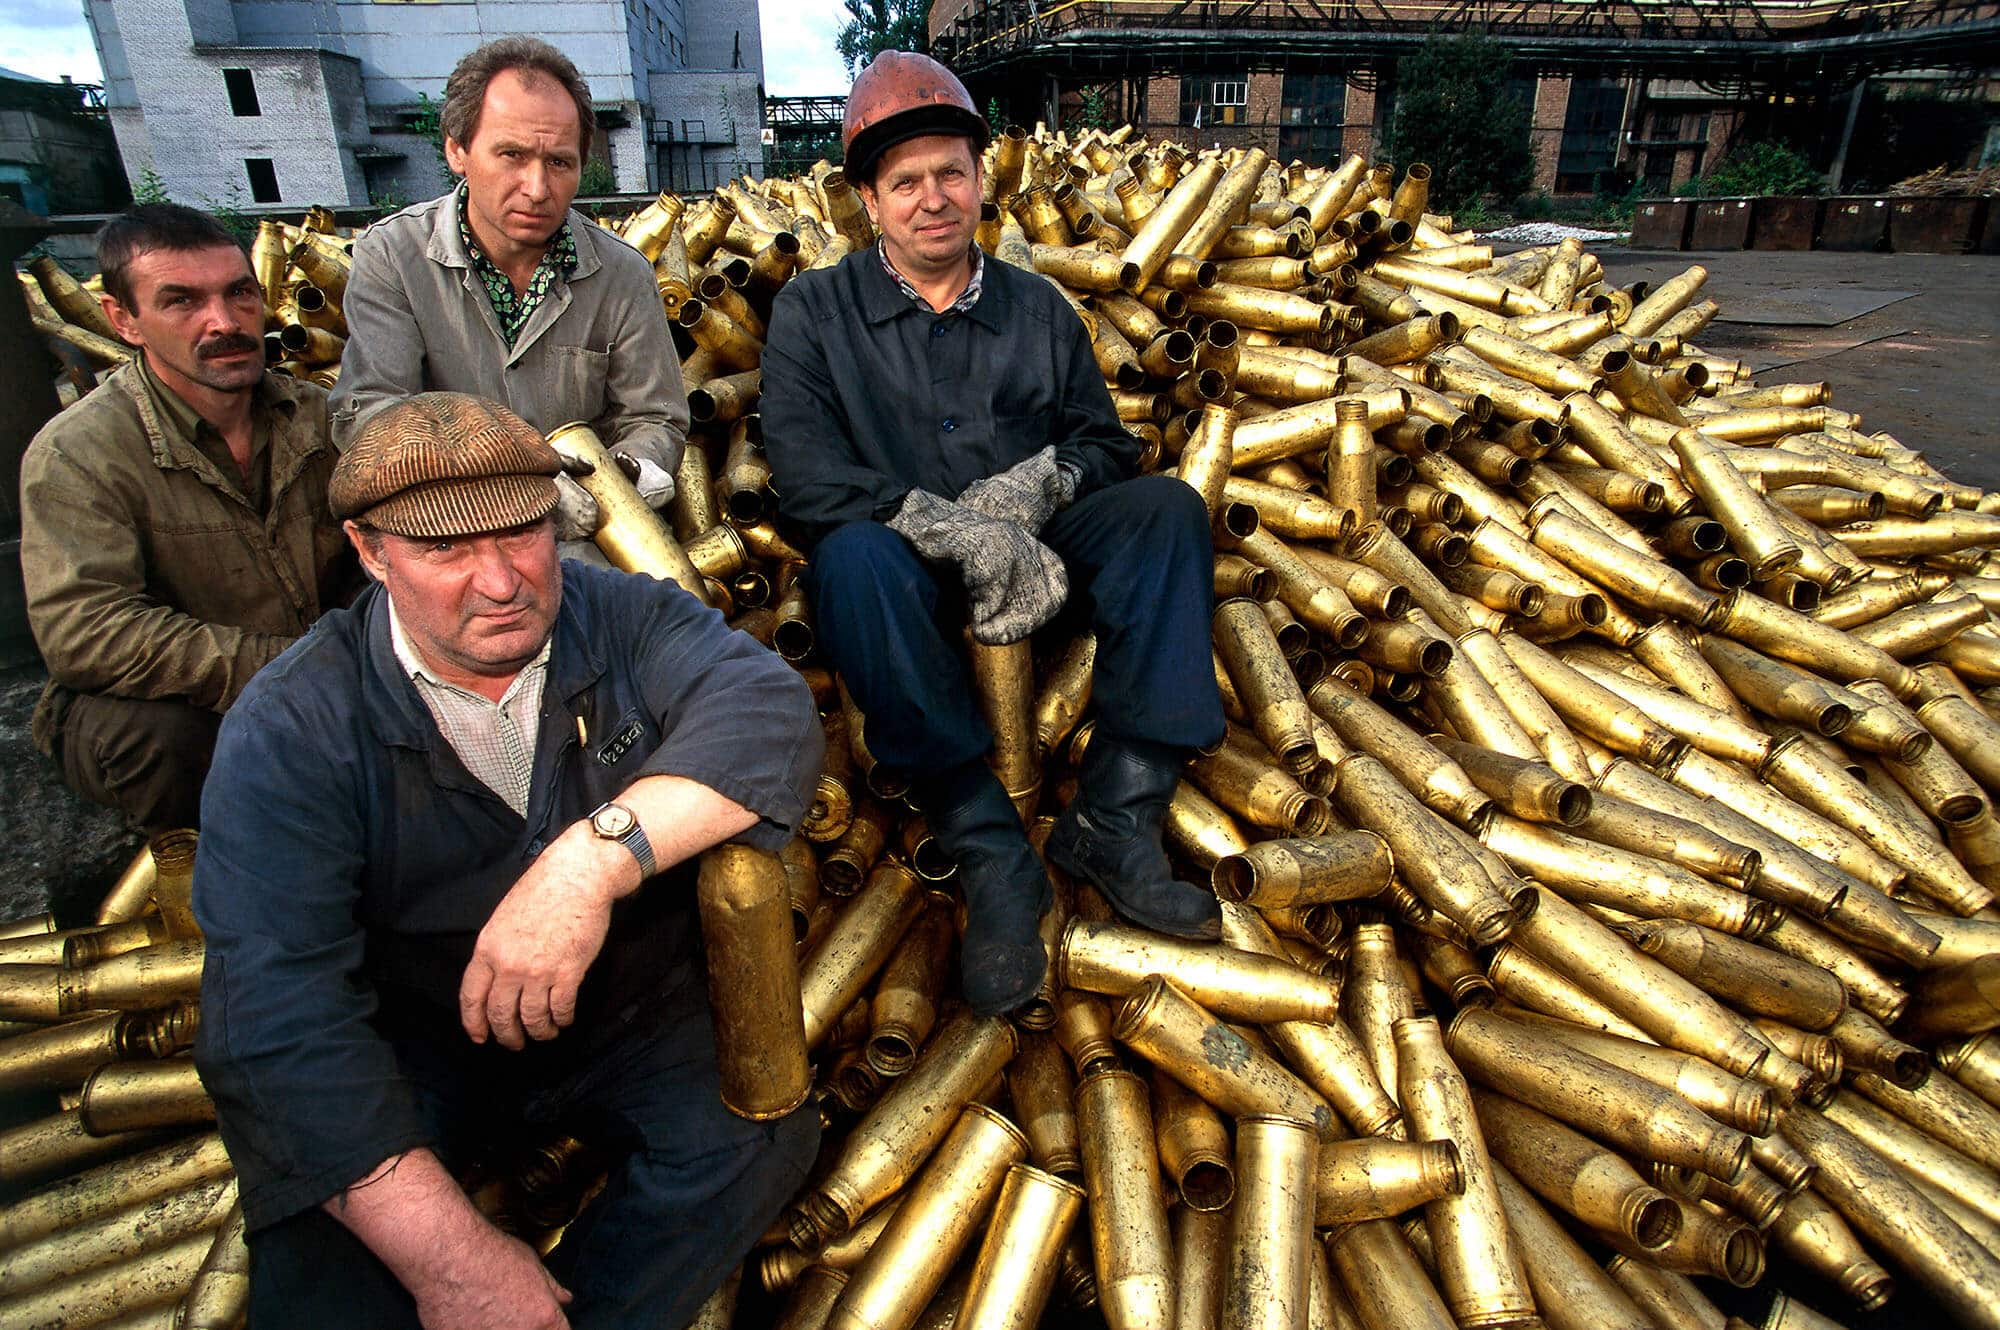
\includegraphics[width=0.45\textwidth,valign=c]{fig/cms/hcal_russian.jpg}\label{fig:cms_hcal_russian}}
    \caption[A photograph of the CMS hadronic calorimeter (HCAL) and the World War II artillery shell casings that were melted down to supply the brass]{
        A photograph of the CMS hadronic calorimeter (HCAL) in front of the magnet and muon chambers before the detector was installed in the experiment cavern (left), from Ref.~\cite{Brice:1431485}, and workers in Mormansk sitting on the decommissioned World War II artillery shell casings used to supply the brass for the HCAL (right), from Ref.~\cite{GinterRussianDudes}.
    }
\end{figure}

\subsection{Muon chambers}
The CMS muon system (Fig.~\ref{fig:cms_subdetector_layout}) was originally composed of three different kinds of detectors: drift tubes (DTs) in the barrel, cathode strip chambers (CSCs) in the endcaps, and resistive plate chambers (RPCs) interwoven between the layers of DTs or CSCs. 
All of the different types of muon chambers operate on a similar principle: muons pass through a chamber filled with gas, liberating electrons from the gas atoms; those electrons are then collected on a conductive surface, resulting in an electric signal~\cite{CERN-LHCC-97-032}. 
The DTs (Fig.~\ref{fig:cms_muon_DT}) and CSCs are assembled into multiple layers that serve as an enormous outer tracker (Fig.~\ref{fig:cms_muon_stations}) exclusively for muons. 
DT and CSC modules also both have multiple inner layers in order to give a measurement of a muon's outer track accurate enough to be matched to its inner track in the silicon tracker. 
The RPCs, meanwhile, are designed to give a much faster, if less accurate, measurement of each muon's momentum. 
This measurement can be used to determine whether the pp collision is interesting or not.

\begin{figure}[htb]
    \centering
    \subfloat[]{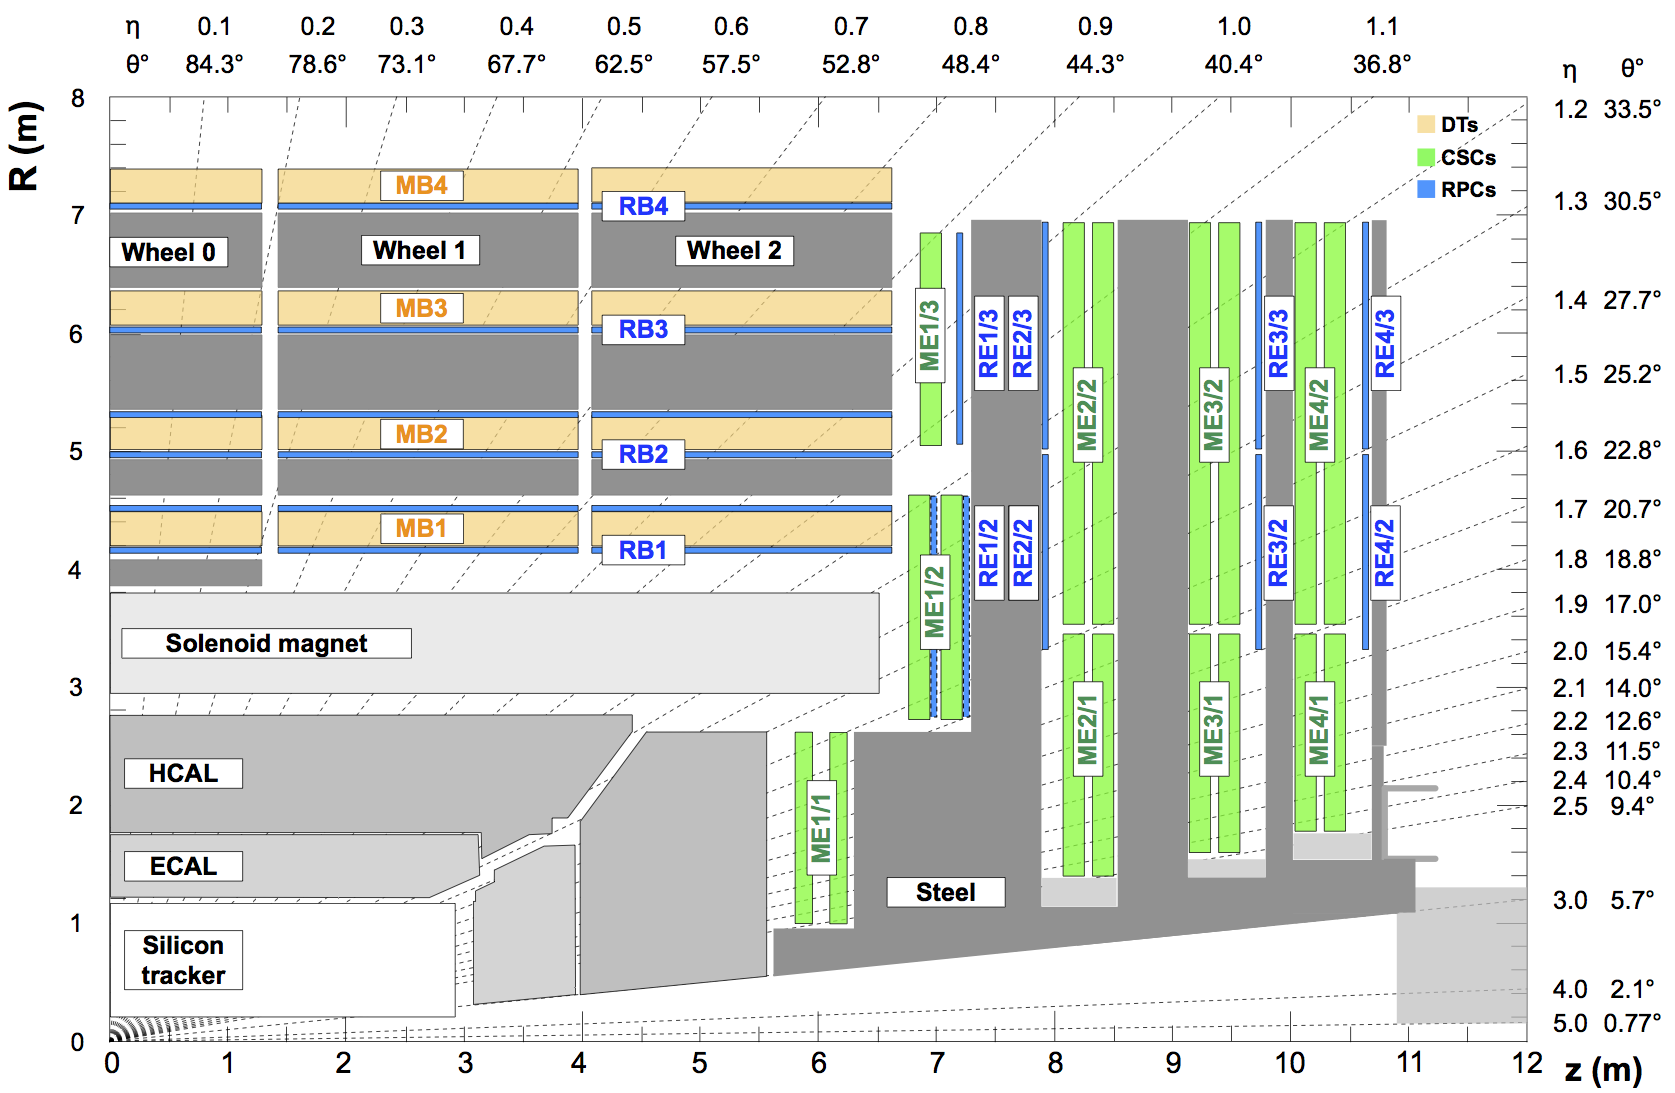
\includegraphics[width=0.6\textwidth,valign=c]{fig/cms/subdetector_layout.png}\label{fig:cms_subdetector_layout}}\quad
    \subfloat[]{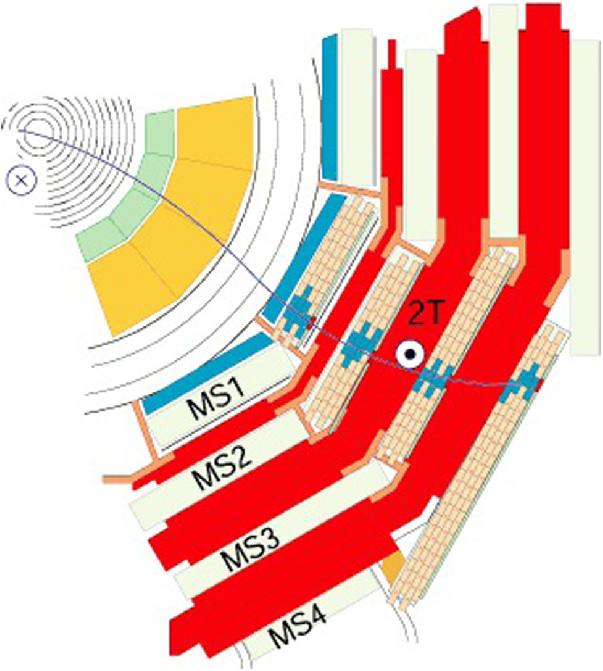
\includegraphics[width=0.3\textwidth,valign=c]{fig/cms/muon_stations.png}\label{fig:cms_muon_stations}}
    \caption[The cross-section of CMS in the $r$-$z$ plane, from Ref.~\cite{CMS:2018rym}, and $r$-$\phi$ plane, from Ref.~\cite{CMSWebMuons}]{
        The cross-section of CMS in the $r$-$z$ plane (left), from Ref.~\cite{CMS:2018rym}, and $r$-$\phi$ plane (right), from Ref.~\cite{CMSWebMuons}. 
        In the $r$-$z$ plane, the DTs, CSCs, and RPCs are drawn in light green, dark green, and blue, respectively, showing the layout of the muon system as well as the other subdetectors. 
        In the $r$-$\phi$ plane, the muon ``stations'' in the barrel are depicted with the DT internals exposed for stations with a throughgoing muon, showing the activation of the individual DT cells (blue) as well as the activation of a section of the RPC (red).
    }
\end{figure}

\begin{figure}[htb]
    \centering
    \subfloat[]{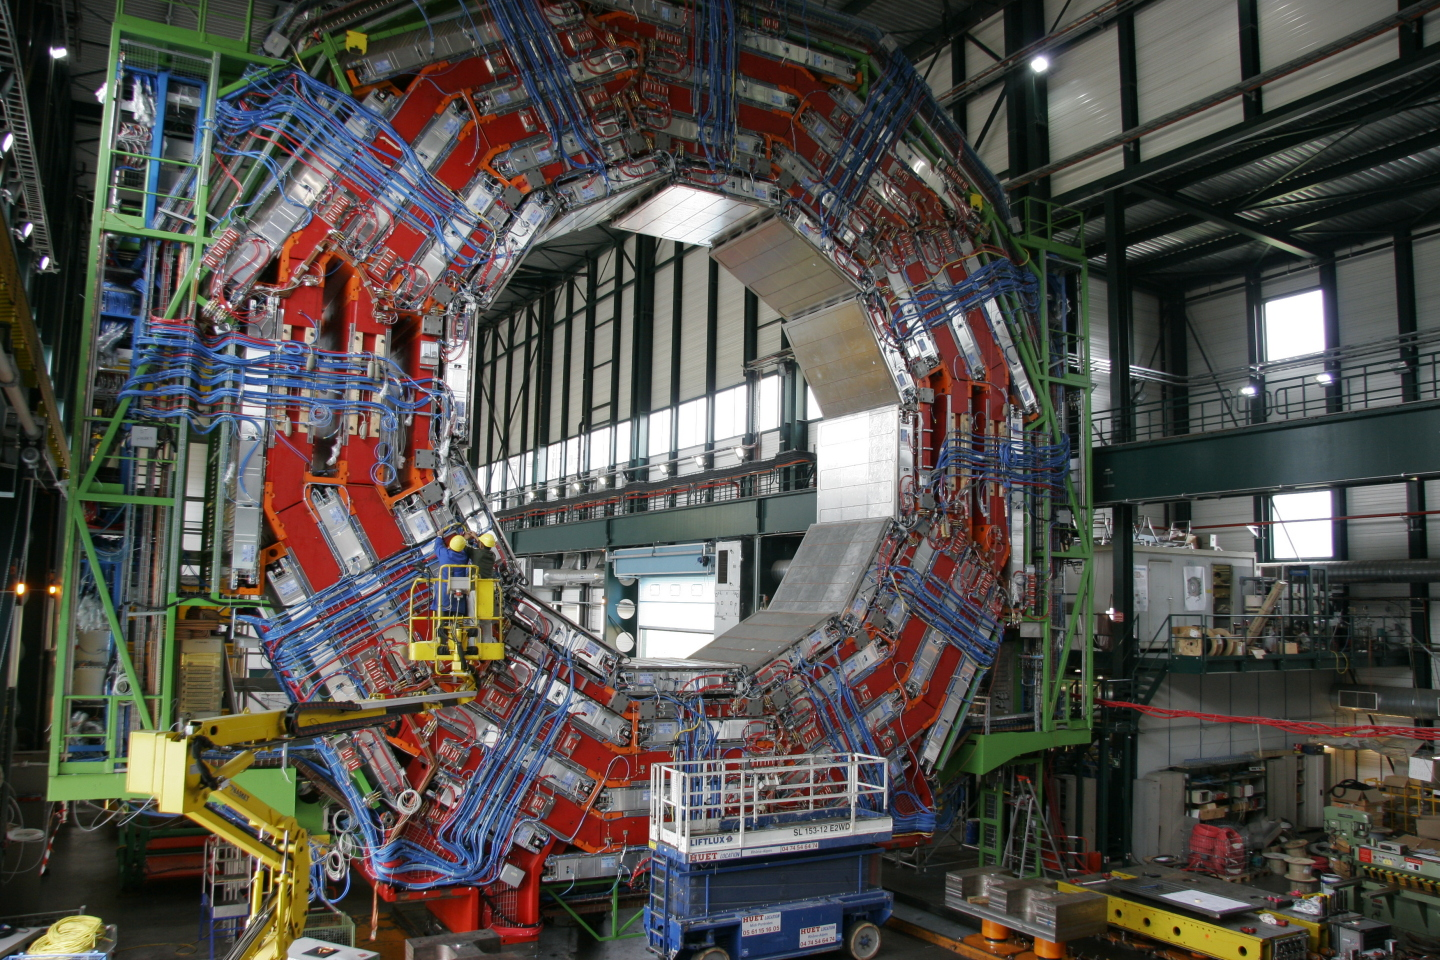
\includegraphics[width=0.465\textwidth,valign=c]{fig/cms/muon_DT_section.jpg}\label{fig:cms_muon_section}}\quad
    \subfloat[]{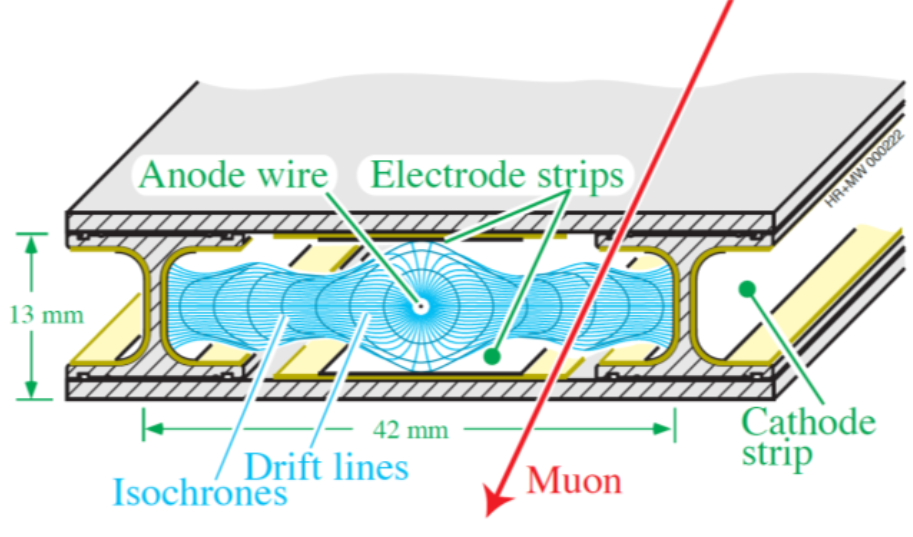
\includegraphics[width=0.435\textwidth,valign=c]{fig/cms/muon_DT_diagram.png}\label{fig:cms_muon_diagram}}
    \caption[A photograph of a section of the barrel muon chambers and a diagram of a drift tube muon detector]{
        A photograph of a section of the barrel muon chambers (drift tubes) before they were installed (left), from Ref.~\cite{Hoch:1274451}, and a diagram of a drift tube muon detector (right), from Ref.~\cite{CMSWebMuonDT}. 
    }
    \label{fig:cms_muon_DT}
\end{figure}

\section{Trigger system}
With bunch crossings every 25 ns, the CMS Experiment would produce 30 terabytes per second (TB/s) if every bunch crossing was recorded. 
Within 24 hours, CMS alone would produce over 2 \textit{exabytes} of data---within a week, CMS could thus easily overwhelm CERN's storage capacity. 
However, pp collisions rarely produce something worth studying like a Higgs boson, vector boson (\PW or \PZ), or something new, which had better be rare, else we should have seen it already. 
We can therefore discard most of the data recorded by CMS, making its continued operation sustainable. 

The CMS Experiment has a two-stage trigger system for identifying interesting events. 
The first stage, called the ``Level 1'' (L1) trigger, takes raw data from the calorimeters and muon chambers and makes a decision on whether to keep or discard the event. 
It is implemented with dedicated hardware (FPGAs), so it can run synchronously with the pp collisions. 
Although it can only make very simple decisions, the L1 trigger reduces the output of CMS from 40 million events per second down to 100\,000 by discarding events that are obviously uninteresting. 
The second stage, called the ``high level'' trigger (HLT), relies on high-throughput software (written in C++), rather than specialized hardware, to reduce the event rate from 100\,000 events per second to 1\,000. 
The HLT is designed to ingest more sophisticated input and thus make more precise decisions. 
In particular, events are processed along trigger ``paths,'' representing different sets of selections. 
Passing events are then sorted and written to disk for further processing. 

\section{The high luminosity era}
There are three primary knobs to turn at the LHC: what things are being collided, what energy they are collided at, and how many of them are collided at once, or the luminosity. 
Since most of the experiments serviced by the LHC were designed for pp collisions, and because the LHC is designed only for $\sqrt{s} = 14\TeV$, the final era of LHC physics will see a massive increase in luminosity. 
That is, at the ``high luminosity'' LHC (HL-LHC), there will be 100--200 concurrent pp collisions per bunch crossing (Fig.~\ref{fig:high_pu}), corresponding to an increase by a factor of 5--7.5.
More collisions mean more opportunities for interesting physics. 
For example, in 2017, the LHC produced 3 million Higgs bosons per year, whereas the HL-LHC will produce over 15 million per year~\cite{HighLumiWebFacts}. 

\begin{figure}[!htb]
    \centering
    \subfloat[]{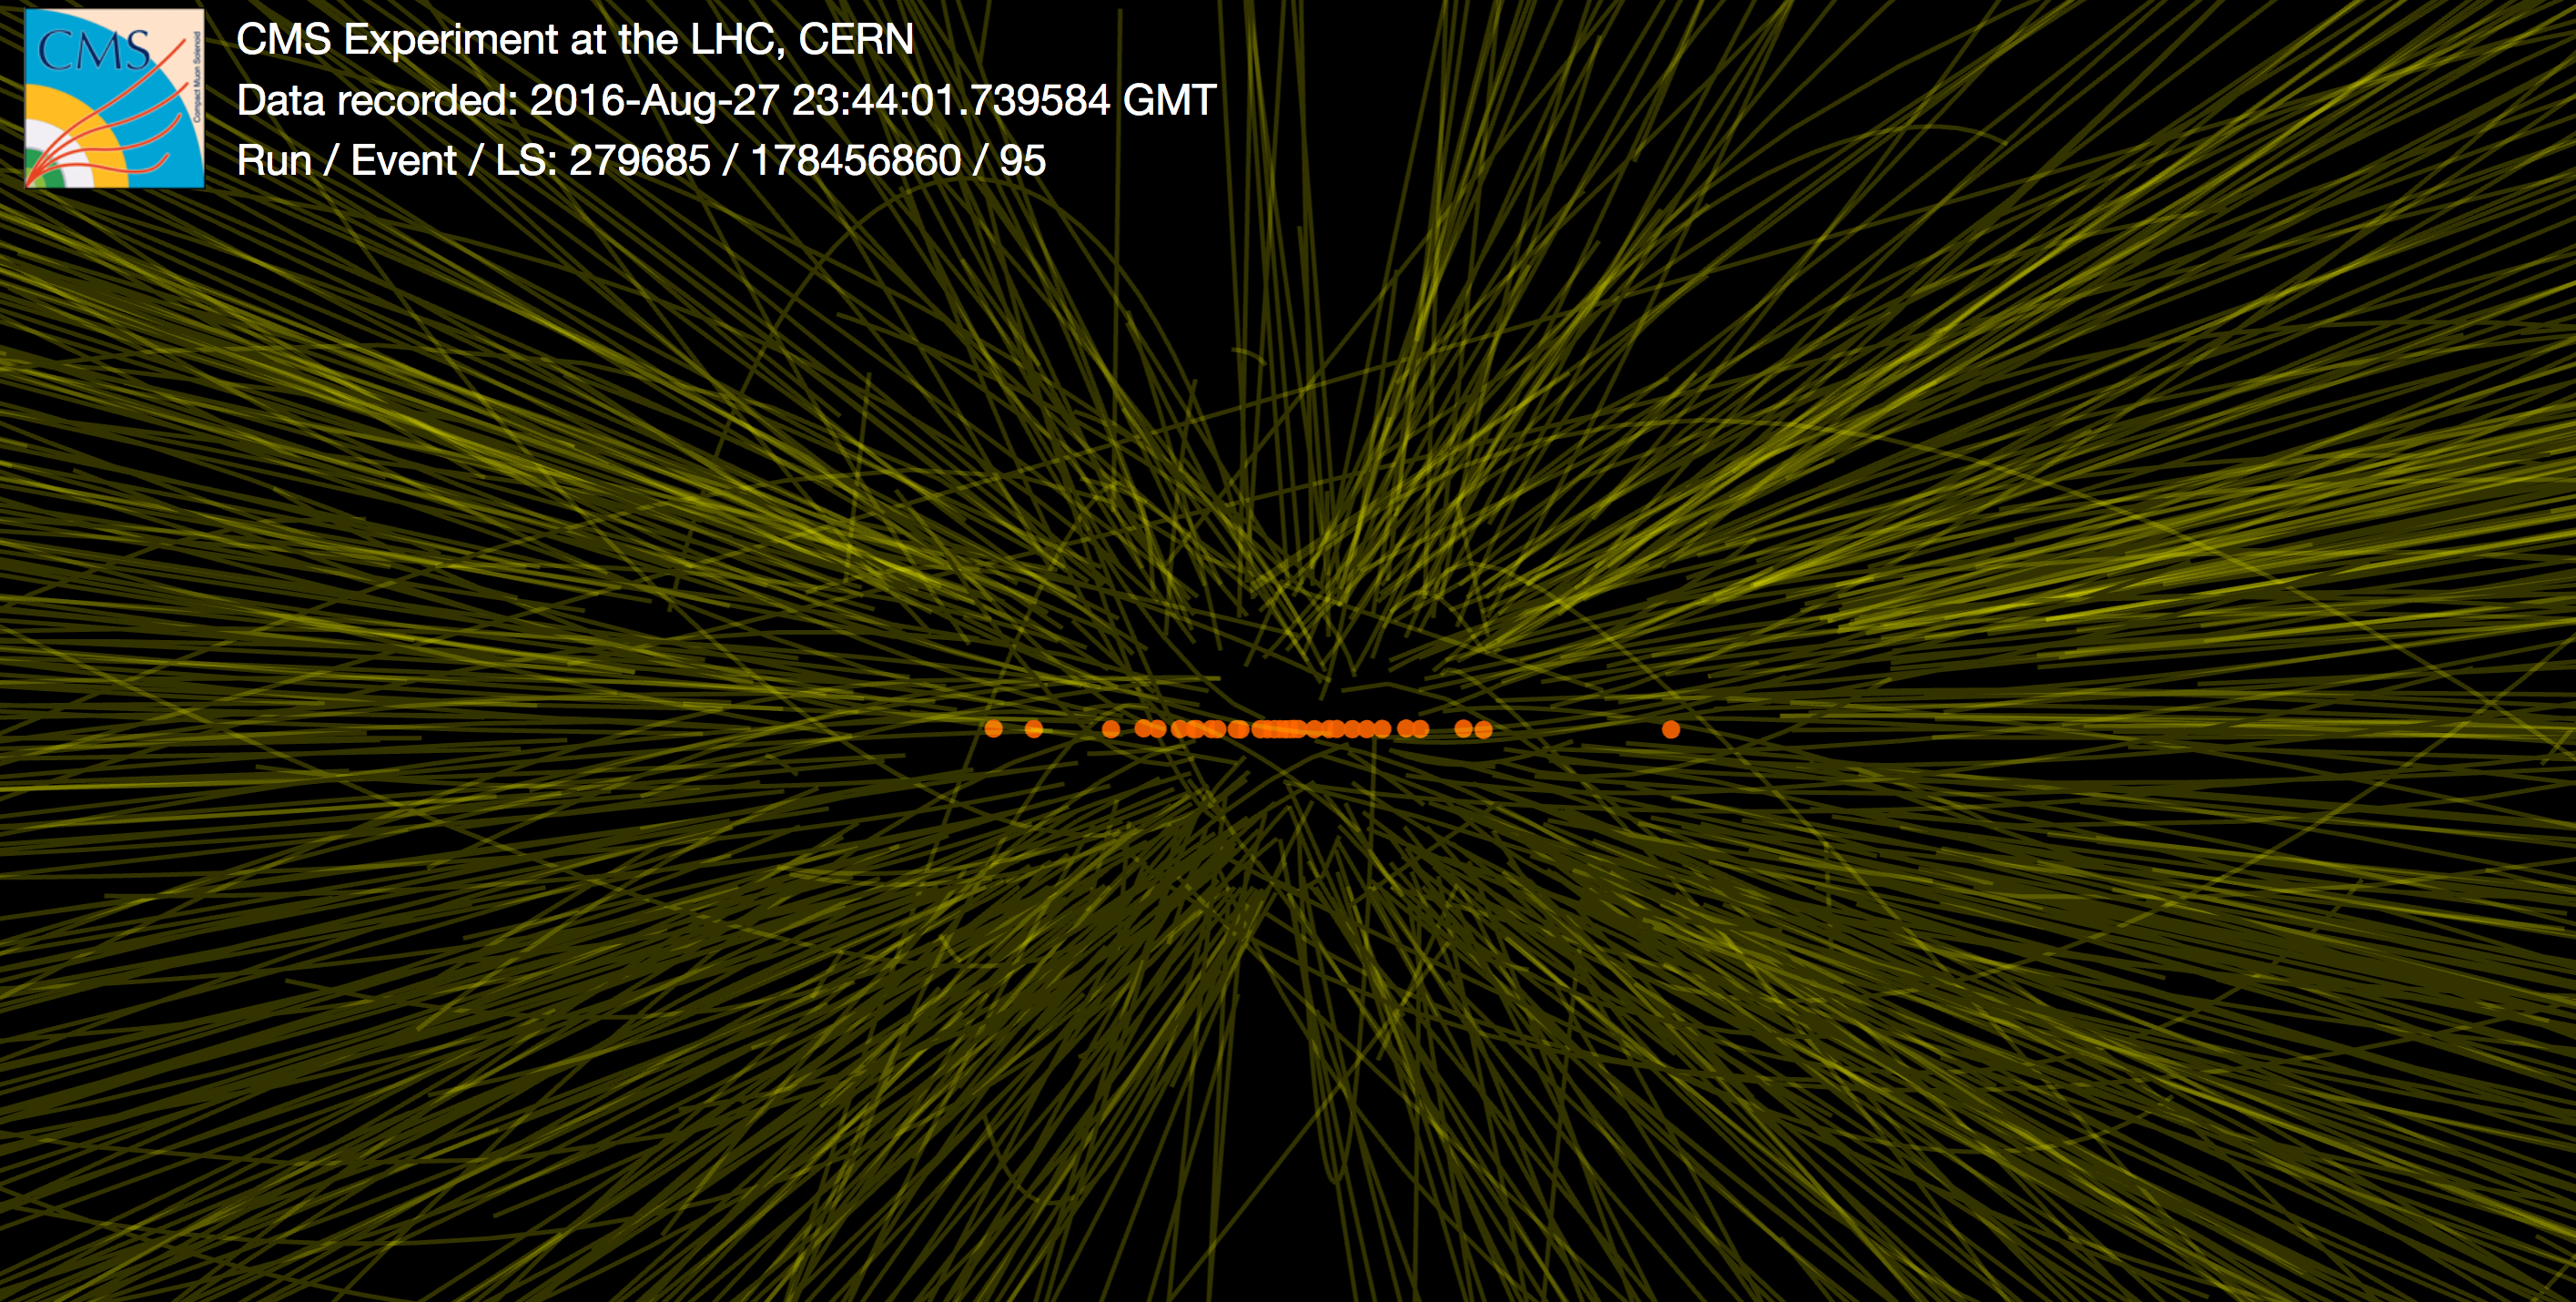
\includegraphics[width=0.45\linewidth]{fig/cms/high_PU_30vtx_side.png}\label{fig:normal_pu}}\qquad
    \subfloat[]{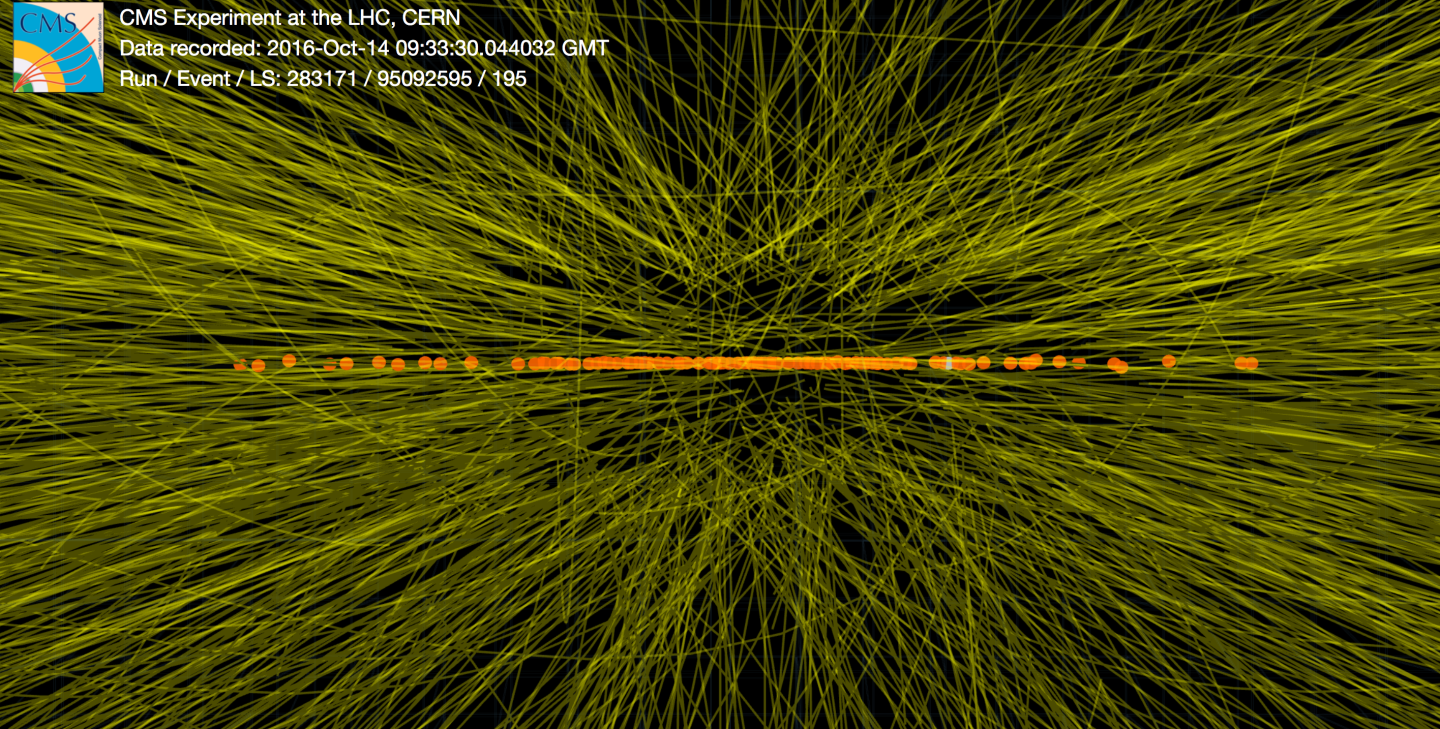
\includegraphics[width=0.45\linewidth]{fig/cms/high_PU_130vtx.png}\label{fig:high_pu}}
    \caption[A collision event with standard pileup and with HL-LHC-like pileup, both recorded in 2016]{
        A collision event with standard pileup (a) recorded at CMS in 2016 is shown next to an event with HL-LHC-like pileup (b) recorded at CMS in the same year, from Refs.~\cite{NormalPU2016, HighPU2016}.
        The dots are pp collisions and the thin lines are the reconstructed particle tracks.
    }
    \label{fig:pileup}
\end{figure}

Significant modifications to the LHC as well as its experiments are needed to enable HL-LHC operations. 
The CMS Experiment, in particular, will receive several upgrades: 
\begin{itemize}
    \item{
        \textit{Enhanced silicon tracker}~\cite{CERN-LHCC-2017-009}: 
        The tracking modules in the outer tracker will be replaced with bilayer modules that give an approximation of a throughgoing particle's \pt. 
        These modules will give the L1 trigger new information as well as provide an opportunity for an entirely new paradigm for offline track reconstruction (Ch.~\ref{ch:lst}). 
    }
    \item{
        \textit{Timing detector}~\cite{CERN-LHCC-2017-027}: 
        A new detector will be added between the tracker and ECAL that provides a precise measurement of when each particle passed through it. 
        This effectively adds another dimension (time) to particle identification, allowing for greater mitigation of pileup. 
    }
    \item{
            \textit{High granularity calorimeter}~\cite{CERN-LHCC-2017-023, CERN-LHCC-2017-011}: 
        The forward sections of the ECAL and HCAL will be entirely replaced with a new calorimeter that incorporates layers of silicon detectors. 
        This will give timing information for PU mitigation, higher resolution, and more. 
    }
\end{itemize}
The muon chambers and trigger system will also see significant upgrades, along with a major overhaul of much of the less glorious hardware.

\section{Acknowledgements}
The figures used in this chapter are materials produced by or for CERN and were released by CERN for informational use under CERN copyright~\cite{CERNCopyright}. 
